\documentclass[]{aiaa-tc} % insert '[draft]' option to show overfull boxes

 \title{Computing Automatic Analytic Gradients for Sparse Multidisciplinary Optimization in OpenMDAO}

\author{
  Justin Gray%
     \thanks{Aerospace Engineer, MDAO Branch, Mail Stop 5-11, AIAA Member},
  \ Tristan A. Hearn,%
     \thanks{Aerospace Engineer, MDAO Branch, Mail Stop 5-10, AIAA Member}
  \ Kenneth T. Moore,%
     \thanks{Senior Systems Engineer, MDAO Branch, Mail Stop 5-11, AIAA Senior Member}
   \\
  {\normalsize\itshape
  NASA Glenn Research Center, Cleveland, OH}  \\
  John T. Hwang,%
  \thanks{Ph.D. Candidate, Department of Aerospace Engineering, AIAA Student Member}
  \ Joaquim R. R. A. Martins%
  \thanks{Associate Professor, Department of Aerospace Engineering, AIAA Associate Fellow}
  \\
  {\normalsize\itshape
   University of Michigan, Ann Arbor, MI}\\
  S. Andrew Ning
    \thanks{Senior Engineer, National Wind Technology Center, AIAA Member}
  \\
  {\normalsize\itshape
   National Renewable Energy Laboratory, Golden, CO}
}

\AIAAconference{Multidisciplinary Design Optimization Specialist Conference}
\AIAAcopyright{\AIAAcopyrightD{2012}}


% Define commands to assure consistent treatment throughout document
\newcommand{\eqnref}[1]{(\ref{#1})}
\newcommand{\class}[1]{\texttt{#1}}
\newcommand{\package}[1]{\texttt{#1}}
\newcommand{\file}[1]{\texttt{#1}}
\newcommand{\BibTeX}{\textsc{Bib}\TeX}

\setlength{\abovecaptionskip}{0pt}
\setlength{\belowcaptionskip}{0pt}

\usepackage{setspace}

\usepackage{graphicx}
\usepackage{wrapfig}
\usepackage{caption}
\usepackage{amsmath}
\usepackage{lscape}
\usepackage{hyperref}
\usepackage{minted}
\usepackage{color}
\usepackage{appendix}
\usepackage{listings}
\usepackage[section]{placeins}
\usepackage[superscript]{cite}
\usepackage{esdiff}
\usepackage{bm}
\usepackage{booktabs}

\lstset{frame=single}
\newcommand{\txt}{\textrm}

\newcommand{\cent}{{\mathrm{c}\mkern-6.5mu{\mid}}}


\captionsetup[figure]{margin=5pt,font=small,labelfont=bf,textfont=bf,justification=justified,}
%\captionsetup[wrapfigure]{margin=5pt,font=small,labelfont=bf,justification=justified,singlelinecheck=off}
\captionsetup[table]{margin=5pt,font=small,labelfont=bf,textfont=bf,justification=justified,position=top}

\bibliographystyle{aiaa}

\usepackage{lettrine}
\usepackage{verbatim}

\begin{document}

  \maketitle

  \begin{abstract}


  Modern design problems often require highly multidisciplinary system level models composed of tens of disciplines. OpenMDAO, 
  a model integration framework, was developed to help facilitate the creation of such models. Traditionally, when gradient 
  based optimization is applied to such large models, finite difference is used to compute system level derivatives. 
  However, as the complexity and size of design problems continue to grow, the computational cost and numerical challenges of 
  from finite difference become prohibitive. Analytic derivatives are an effective solution for solving large scale design 
  optimizations, but computing system level analytic derivatives for large multidisciplinary models inside a framework is challenging. 
  To address this challenge a method was developed to efficiently computing analytic and semi-analytic derivatives for sparse multidisciplinary
  models inside the OpenMDAO framework, given discipline level partial derivatives. A graph-based representation of 
  problem formulation was utilized to detect and efficiently handle sparsity at the problem formulation level. 
  Additionally, a flexible API was built for declaring discipline-level derivatives to handle sparsity within a the Jacobian for a specific discipline. 
  The combined approach yielded an efficient and flexible tool that solved system-level forward and adjoint derivatives 
  for two different example problems. First A small satellite design optimization was performed, using analytic adjoint gradients, to maximize the 
  information transfered to a ground station over the course of a year. This problem demonstrated a significant computational cost reduction for
  the graph-based approach to computing derivatives. Second a wind turbine design optimization was run using mixed analytic and 
  finite-difference forward derivatives. The results showed improved convergence and reduced computational cost for mixed derivatives. 
  Overall the results show that OpenMDAO can efficiently compute derivatives for a wide range of problems with large design spaces and 
  complex problem formulations and demonstrate the advantage of implementing analytic derivatives even for only parts of the problem.

  \end{abstract}

  \section{Introduction}

    Gradient-based optimization with analytic gradients is an effective tool for solving problems
    with large design spaces. It has been applied widely for aerodynamic shape optimization \cite{Liou2010,palacios2012adjoint}
    and structural optimization\cite{Kennedy:2013:TACS, Venkataraman:2004:SOC, Adelman:1986:structure-sensitivity}.
    To apply these methods to multidisciplinary problems, system-level derivatives must be
    constructed by combining the partial derivatives from each discipline using the Global Sensitivity
    Equations\cite{Sobieski1990} (GSE). This technique is commonly applied to coupled
    aero-structural design optimization of aircraft wings\cite{Kenway2012c, Haghighat2012} and is applicable to
    other multidisciplinary design problems such as aero-acoustic design\cite{economon2012coupled}. Extending these
    gradient-based techniques to more complex problem formulations has proved difficult. When
    design problems grow to include tens of disciplines, it becomes increasingly challenging to construct the
    necessary derivatives. Even assuming all of the disciplines provide analytic partial derivatives,
    constructing the system-level derivatives depends heavily on the structure of the data connections
    between disciplines. Manual implementations for these problems are time consuming and discourage modifications
    to the problem formulation in the future. To overcome these issues, Moore developed a method for automatically assembling the system
    level derivatives based on the data-dependency graph of a given problem formulation\cite{openmdao_derivatives}. This
    work represented the first implementation of Martins and Hwang's unified approach to computing system-level derivatives,
    which combined forward- and adjoint-based derivatives into a single theoretical framework\cite{martins2013}.
    In addition to allowing greater flexibility in the problem formulation, a key feature of Moore's graph-based approach was the efficient
    handling of sparse problem formulations. By traversing the graph from design variables to quantities of interest,
    it was possible to consider only the subset of variables that were relevant to a specific system-level gradient, thus
    making gradient computations more efficient.

    Although Moore's work demonstrated that a framework could compute system-level derivatives for arbitrary
    problem setups, the implementation assembled and inverted a complete system-level Jacobian for
    all derivative solves.  This approach made it unsuitable for larger problems involving
    high-fidelity tools, since enumerating a full Jacobian would be inefficient (if possible at all).
    Hwang et al. developed an alternative, graph-free method for computing automatic system
    level sensitivities which used a global design variable vector\cite{CADRE2012}. Their method
    addressed the scalability challenges with Moore's work by using a matrix-free approach with
    components providing partial derivatives via a linear operator. They demonstrated the
    effectiveness of their method on a design optimization of a small satellite
    with over 25,000 design variables and over 1 million state variables. Despite its success,
    the global-vector-based approach required that all the variables from the system model be
    included when solving for system-level derivatives. This prevented the method
    from taking advantage of sparsity in the problem formulation and resulted in a less efficient gradient solving step.

    This work combined the graph-based approach with the matrix-free solution algorithm
    to efficiently compute derivatives for a wide range of sparse, large-scale engineering
    design problems. This new implementation was tested on the same small satellite design problem used in
    Hwang et. al's original work and demonstrated a dramatic reduction in computational cost. In addition,
    the new method was applied to a wind turbine design study that had a more
    complex structure with stronger multidisciplinary couplings as well as a mixture of
    analytic and finite-difference gradients. Comparisons between finite-difference and analytic gradient
    performance were made, demonstrating faster and tighter convergence with analytic gradients.

  \section{Unified Derivatives Computations}

    There are several methods for computing system-level derivatives that differ in accuracy, efficiency, and ease of implementation.
    The black-box finite-difference approximations involve the least amount of implementation effort, but they suffer from accuracy
    limitations caused by the combination of truncation and subtractive cancellation error that become worse with increasing nonlinearity in the model.
    Furthermore, the cost is at best the number of design variables times the cost of evaluating the full multidisciplinary model.
    The complex-step method eliminates the accuracy issue at the cost of increased implementation complexity but is typically 
    two to three times slower than finite difference which is already relatively inefficient.

    The complex-step method can be invasive to a small extent, but the remaining methods typically require an even greater level of source code access and modification.
    Algorithmic differentiation (AD) uses automated tools to symbolically differentiate at the line-of-code level and combine the resulting partial derivatives to obtain numerically exact values for the system-level derivatives.
    AD operates in the forward and reverse modes, with the cost of the former proportional to the number of design variables and the latter to the number of output functions.
    Analytic methods have the same two modes of operation and have the added advantage that only a linear system needs to be solved to obtain a vector of derivatives, which is cheaper than an evaluation of the model in some cases.

    When implementing multidisciplinary problems, derivatives for each individual discipline
    are typically available and must be combined to compute system-level derivatives.
    The manner in which the derivatives are combined is highly problem-dependent.
    If there is no feedback among the disciplines and they are explicit functions, one can simply
    use the chain rule at the discipline-level. If all of the disciplines have residuals from the
    discretization of governing equations, the coupled adjoint or coupled direct method would be
    the most appropriate for computing system-level derivatives. If the disciplines are explicit
    but there is coupling among disciplines, the GSE equations must be used.

    A framework that automatically computes system-level total derivatives from user-provided
    partial derivatives for each discipline must be able to apply the most appropriate method
    for the situation (explicit/implicit, coupled/sequential, etc.). This is greatly facilitated by a
    unification of derivative computation methods using a single equation from which all
    methods can be derived\cite{martins2013}:
    \begin{equation}
        \diffp[]{\bm C}{\bm v} \diff{\bm v}{\bm c} = \mathcal{\bm I} = \left. \diffp[]{\bm C}{\bm v} \right.^T \left. \diff{\bm v}{\bm c} \right.^T
    \end{equation}
    where $\bm C$ represents the vector of functions that constrain the variables $\bm v$ to their appropriate values.

    By appropriately choosing $\bm v$ and $\bm C$, chain rule, black-box methods, analytic methods, GSE equations, and algorithmic differentiation can be derived.
    For instance, including only the design variables and output variables in $\bm v$ yields a black-box method because all intermediate variables involved in computing the output variables are ignored in this situation.
    The significance of the above equation is that it enables a much simpler implementation of the derivative computation algorithm in the framework.
    Regardless of the specifics of a given problem, computing derivatives reduces to solving a linear system in the left or right equality of the above equation.

  \section{Dependency Graph}\label{section:depgraph}

    In Moore's original work on computing derivatives from a dependency graph, he employed
    a discipline-based dependency graph, with a node for each discipline and edges describing
    dependency between the nodes. A path-finding algorithm, from the NetworkX library\cite{hagberg-2008-exploring},
    computed the relevant set of disciplines for a given derivative. Although the dependency-based graph took advantage of sparsity at
    one level, by excluding any disciplines that did not directly contribute, it did not handle a second level of sparsity
    within disciplines. Even if a given discipline is relevant, some of its variables still may not
    directly affect the quantities of interest. To handle this problem, Moore utilized a secondary source of information
    outside the dependency graph. Pate et al. proposed an alternative dependency graph
    structure that addressed this problem\cite{graph_problem2013}. Each discipline and each of its variables are
    represented by separate nodes with directed edges between them describing their dependencies on each other.
    Figure \ref{fig:sample_graph_full} shows a sample graph for a notional problem formulation. 

    \begin{figure}[!htb]\begin{center}
      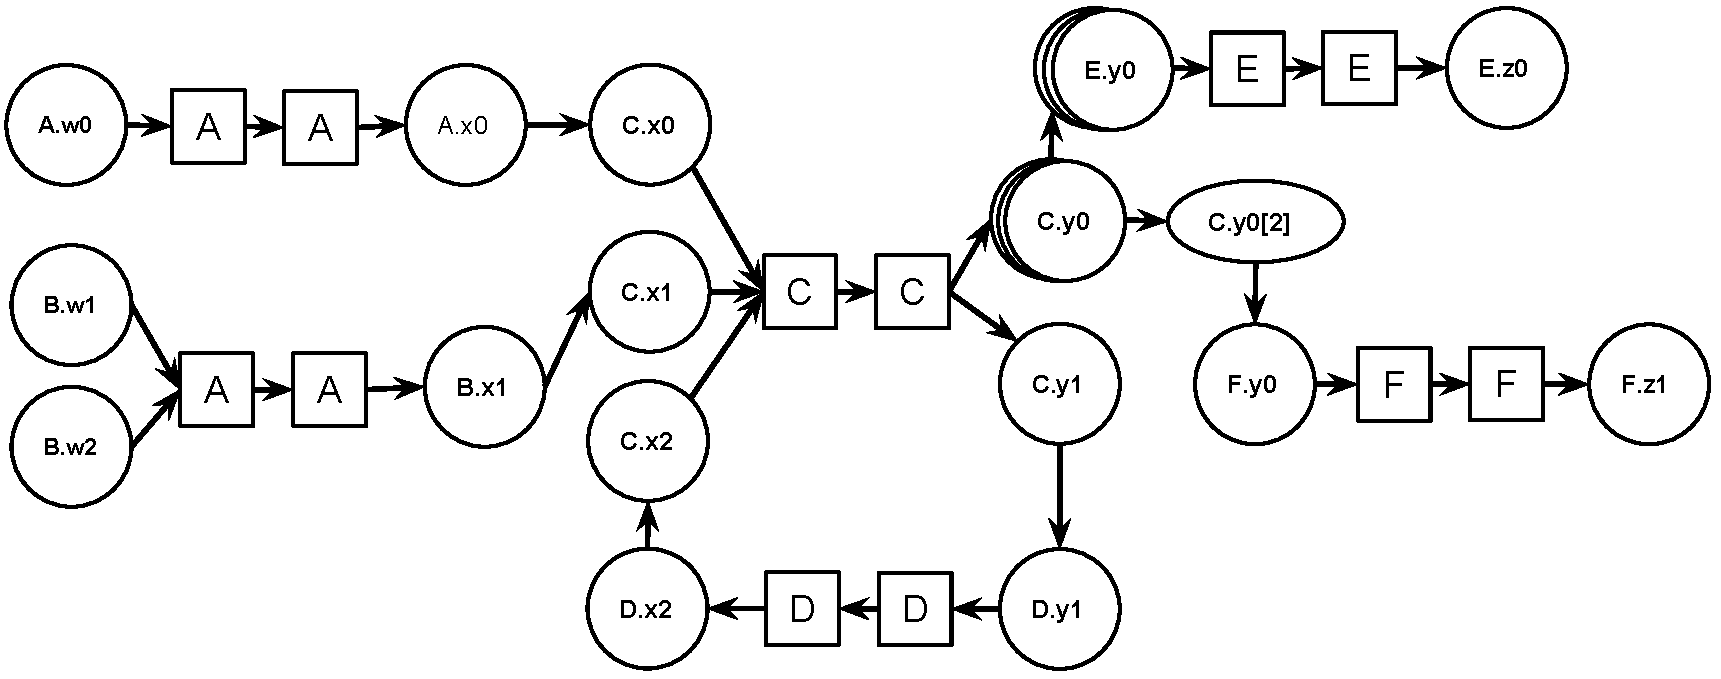
\includegraphics[width=.8\textwidth]{images/sample_graph_full}
      \caption{ Dependency graph for a notional problem, using Pate et. al's proposed structure\label{fig:sample_graph_full}}
    \end{center}\end{figure}

    In Pate et al.'s graph syntax, a single node is given for every variable, and two nodes are given
    for each discipline analysis. The dual discipline nodes were prescribed in order to create an edge
    that could be assigned a weight in case weighted graph traversal algorithms were desired. However,
    they acknowledged that the dual nodes are often unnecessary and could be avoided for the sake of simplicity.
    Figure \ref{fig:sample_graph} shows the same notional problem, with the simplification of using only single 
    model nodes made. 

    \begin{figure}[!htb]\begin{center}
      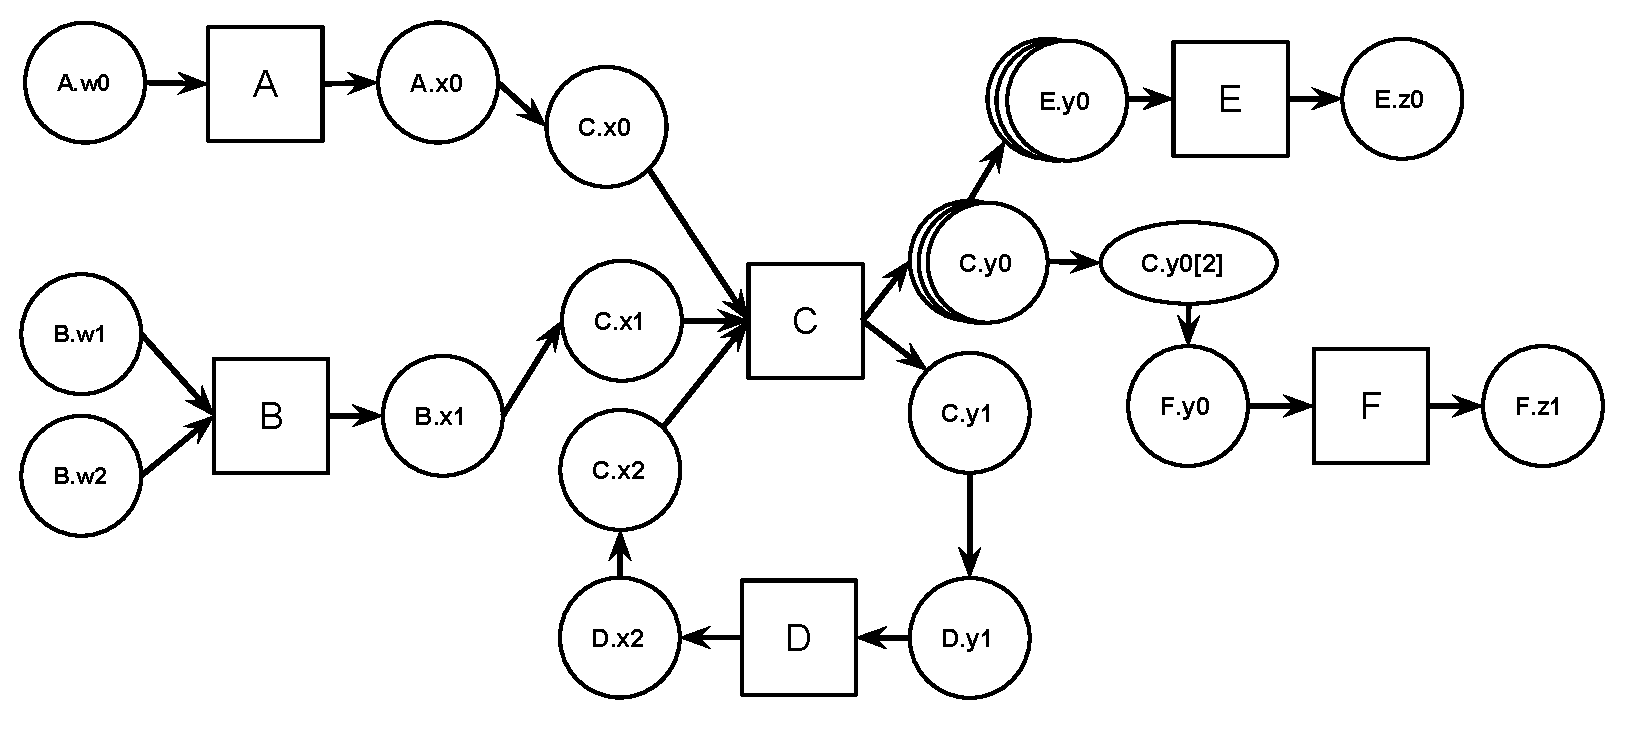
\includegraphics[width=.8\textwidth]{images/sample_graph}
      \caption{Dependency graph for a notional problem, using Pate et. al's proposed structure with a only one model node \label{fig:sample_graph}}
    \end{center}\end{figure}


    This graph contains all the information needed to take full advantage of problem sparsity but suffers from one potential
    weakness. For a problem with millions of  variables, like the small satellite design problem,
    the graph would get very large and would be inefficient to operate on. To address this issue,
    related variables (i.e., arrays) can be aggregated into a single node to represent the
    overall variable. For problems with large arrays, this modification results in a significant reduction
    in the overall size of the graph. If any specific subvariable is referenced (e.g., some slice of an array)
    then a new node is added to represent that relationship. In Fig. \ref{fig:sample_graph} variable nodes C.y0 and E.y0 are both 
    arrays and are directly connected. However F.y0 is a scalar variable, which depends on a single entry form C.y0, 
    so a subvariable node, C.y0[2], is added to the graph inbetween C.y0 and F.y0. 
    By using the subvariable nodes, the computational advantages of problem sparsity are retained. Consider 
    $\frac{\partial F.z1}{\partial C.y0}$. Given the graph, we know that
    this gradient will be sparse, with only the element relating to C.y0[2] having nonzero values as in Eq. \ref{eqn:sparse_gradient}.

    \begin{equation}
        \frac{\partial B.z}{\partial A.y} =
        \begin{bmatrix}
            0 \\
            0 \\
            \frac{\partial B.z}{\partial A.y[2]} \\
            \vdots \\
            0 \\
        \end{bmatrix}
        \label{eqn:sparse_gradient}
    \end{equation}

    Because of the variable aggregation, solving for derivatives without the subvariable node would require
    all the elements of the C.y0 array to be included in the linear system.
    With the subvariable node, only the single relevant value from the array needs to be included.
    By representing hierarchical data as a single node the overall size of the graph
    remains manageable and the subvariable nodes are used to preserve the benefits of sparsity.


    \subsection{Graph Traversal Determining Relevance}
    \label{sec:determing relevance}

        OpenMDAO can calculate a gradient between any set of input and output nodes in a
        model by setting up the appropriate linear system. The size of the linear system
        is determined by the number of variables being considered, which means that the linear
        system can get very large. Although the matrix-free approach to solving this system
        can handle larger problems well, it is still desirable to minimize the size of the problem
        as much as possible. OpenMDAO was able to achieve significant reductions in the
        size of the linear system by traversing the dependency graph to find the subset of relevant variables.
        Consider solving for the derivative of $\frac{\partial F.z1}{\partial A.w0}$, given Fig. \ref{fig:sample_graph}. 
        Figure \ref{fig:graph_relevance_path} highlights the relevant path through thre graph between A.w0 and F.z1. 
        Only components A, C, D, and F are needed. Furthermore, only C.x0 and C.x2 are needed from C, because of component-level sparsity.
        This means that only seven variables are needed to solve for the derivatives,
        instead of eleven if the graph is not reduced.

        \begin{figure}[!htb]\begin{center}
          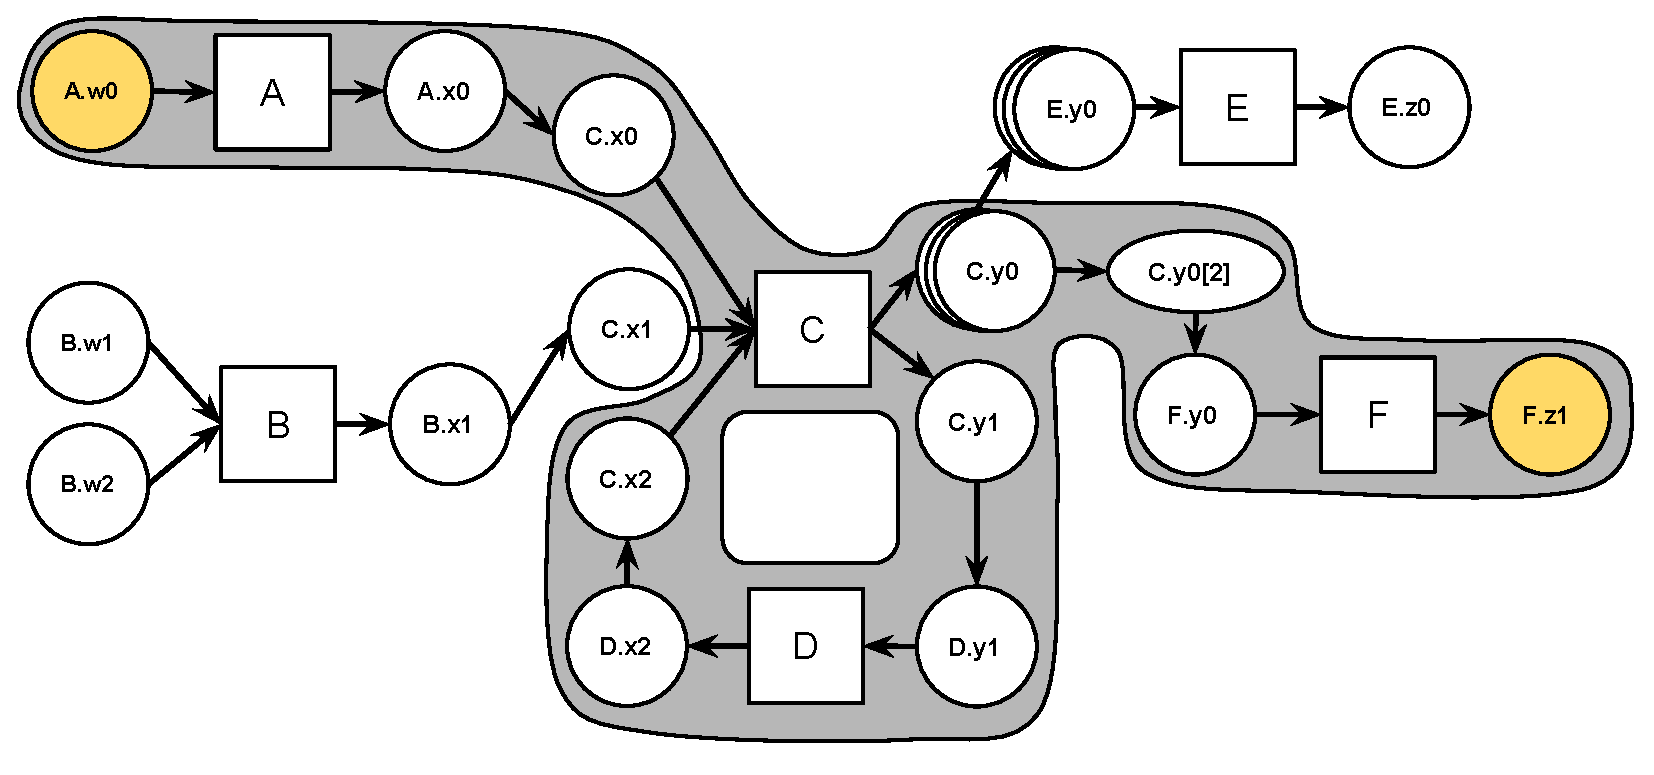
\includegraphics[width=.8\textwidth]{images/sample_graph_path}
          \caption{ The reduced graph for the derivatives calculation includes components 1, 3,
          and 5 with their interconnecting variables. \label{fig:graph_relevance_path}}
        \end{center}\end{figure}

        A traversal from parameter to quantity of interest, as shown in Fig. \ref{fig:graph_relevance_path}, is used when solving for
        forward derivatives. In forward mode, the traversal searches for all of the variables that could possibly
        be affected by a change in the parameter. One traversal is necessary for each design variable in the
        problem formulation. To solve adjoint derivatives, a traversal must be made in
        the opposite direction. To do this, reverse all of the edges in the dependency graph and
        perform one traversal from each quantity of interest to all possible parameters.

    \subsection{Cycle Detection and Usage}
        Pate et al. stated that within a dependency graph, the presence of cycles indicates coupling between
        the components in the cycle \cite{graph_problem2013}. Cycles can be induced by connections
        where data is passed directly from an output to an input, or implicitly where an input needs to
        be varied in order to drive a residual equation to zero. In Fig. \ref{fig:sample_graph} there 
        is a cycle between components C and D. The presence of cycles has
        an impact on how models are solved. First, during normal execution, these cycles
        need to be converged with a numerical solver such as Gauss-Seidel or a Newton-based solver.
        In addition, these cycles need to be accounted for when solving for the derivatives. Martins and Hwang's
        unified gradient method allows for this situation but requires the resulting residual equations be
        handled in a slightly different manner from explicit variable relationships (ones without cycles). Hence
        it is important to be able to efficiently identify all cycles in the graph. In formal terms,
        cycles exist in a graph when a group of nodes are strongly connected. Tarjan's algorithm provides
        an efficient means of finding the sets of strongly connected components\cite{tarjan1972depth,nuutila1994finding}.


    \section{API for Specifying Discipline Derivatives}

        All of the discussion up to this point has dealt with disciplines as if they are black boxes
        which are assumed to provide analytic derivatives of their outputs with respect to their inputs
        to the framework. This section describes the API for components to declare and provide
        said derivatives. The API is broken up into two parts: one that is mandatory for all components
        that declare derivatives, and another that is optional for components that wish to take full
        advantage of the graph-based sparse approach.

        \subsection{Mandatory API Methods}

        There are two mandatory methods that all components supporting derivatives must provide.
        The first is \texttt{list\_deriv\_vars()}. This method specifies the
        input and output variables that make up the columns and rows of its Jacobian, respectively.
        \texttt{list\_deriv\_vars()} returns a 2-tuple of inputs and outputs that have derivatives.
        A component is allowed to declare derivatives support for an arbitrary subset of all its variables.

        The second method is \texttt{provideJ()}. This method serves two purposes. First, it provides the
        opportunity to perform any one-time work needed for linearization around the current point. Second,
        the method can optionally return the actual Jacobian, in the form of a $n \times m$ vector, where $n$ is the
        number of outputs and $m$ is the number of inputs. The ordering of the rows and columns of the Jacobian
        must match the order of the variables returned for \texttt{list\_deriv\_vars()}. When a Jacobian is
        returned from \texttt{provideJ()}, OpenMDAO will cache it and use it for all derivative computations
        around the current point for both forward and adjoint derivatives. This makes the \texttt{provideJ()}
        API the most straitforward and easiest to use in many cases. Figure \ref{fig:code-block-1} shows
        an example of an OpenMDAO component with user-specified derivatives, using the \textit{provideJ()}method.
        This component has two input variables, $x$ and $y$, and two output variables, $f$ and $g$, where

        \begin{align}
            f\left(x, y\right) =&\  x^2 + \sin(y) \\ \notag
            g\left(x, y\right) =&\  x^3
        \end{align}

\begin{figure}
\begin{minipage}{\textwidth}
\begin{lstlisting}[
language=Python, basicstyle=\ttfamily\scriptsize,
           keywordstyle=\color{blue}\ttfamily,
           stringstyle=\color{red}\ttfamily, showstringspaces=false,
           commentstyle=\color{olive}\ttfamily]

from openmdao.main.api import Component
from openmdao.main.datatypes.api import Float
from math import sin, cos
from numpy import array

class ExampleComp(Component):

    # Inputs
    x = Float(0., iotype="in")
    y = Float(0., iotype="in")

    # Outputs
    f = Float(0., iotype="out")
    g = Float(0., iotype="out")

    def list_deriv_vars(self):
        return (('x', 'y',), ('f', 'g'))

    def provideJ(self):
        return array([[2 * self.x, cos(self.y)],
                      [3 * self.x ** 2, 0.0]])

    def execute(self):
        self.f = self.x ** 2 + sin(self.y)
        self.g = self.x ** 3

\end{lstlisting}
\caption{Example of an OpenMDAO
component with user-specified Jacobian.
\label{fig:code-block-1}}
\end{minipage}

\end{figure}

        Although the \texttt{provideJ()} method is easy to implement, it does have a few minor downsides. First,
        it requires that the component Jacobian be assembled in memory. In most cases, with tens or even hundreds of variables
        this is reasonable, but if the Jacobian has a sparse structure, it may still be wasteful to allocate memory for a
        full matrix. Furthermore, for situations like Computational Fluid Dynamics, where there are millions of variables spread out
        across many CPUs, assembling the full Jacobian is simply not feasible. Lastly, depending on how
        your problem is configured, it is possible that not all of the variables will be needed for a given problem, as in Fig. \ref{fig:graph_relevance_path}.
        With \texttt{provideJ()}, the full Jacobian will still need to be provided though some of it will be irrelevant.
        So in effect, using the \texttt{provideJ()} method can partially negate some of the benefits of problem sparsity.
        In general, these inefficiencies are small and easily outweighed by the ease of implementation. But in cases where
        these downsides become a significant concern, the \texttt{provideJ()} method should return nothing, and instead the
        optional API methods should be implemented for improved efficiency.

    \subsection{Optional API Methods}

        To overcome some of the downsides of constructing the full Jacobian, the components can provide
        a linear operator that computes the effect of multiplying the Jacobian with a given vector. This provides
        more freedom in how derivatives are implemented. It also enables the computing of only
        relevant quantities. The only significant downside is a small amount of added implementation complexity.
        Two different methods, \texttt{apply\_deriv(arg, result)} and \texttt{apply\_derivT(arg, result)}, must be implemented
        for forward and adjoint derivatives respectively. In each case, \texttt{arg} and \texttt{result}
        are dictionaries with relevant input and output variable names as keys.
        If only forward or adjoint derivatives will be used, then only the necessary method needs to be implemented. Figure \ref{code:component_with_apply_deriv} provides an example of
        the \texttt{apply\_deriv} and \texttt{apply\_derivT} methods; using the same component shown above in
        Fig. \ref{fig:code-block-1}.


\begin{figure}
\begin{minipage}{\textwidth}
\begin{lstlisting}[
language=Python , basicstyle=\ttfamily\scriptsize,
           keywordstyle=\color{blue}\ttfamily,
           stringstyle=\color{red}\ttfamily, showstringspaces=false,
           commentstyle=\color{olive}\ttfamily]

class ExampleComp(Component):

    # Inputs
    x = Float(0., iotype="in")
    y = Float(0., iotype="in")

    # Outputs
    f = Float(0., iotype="out")
    g = Float(0., iotype="out")

    def list_deriv_vars(self):
        return (('x', 'y',), ('f', 'g'))

    def provideJ(self):
        pass

    def apply_deriv(self, arg, result):
        if "x" in arg:
            result["f"] += 2 * self.x * arg["x"]
            result["g"] += 3 * self.x ** 2 * arg["x"]
        if "y" in arg:
            result["f"] += cos(self.y) * arg["y"]


    def apply_derivT(self, arg, result):
        if "f" in arg:
            result["x"] += 2 * self.x * arg["f"]
            result["y"] += cos(self.y) * arg["f"]
        if "g" in arg:
            result["x"] += 3 * self.x ** 2 * arg["g"]

    def execute(self):
        self.f = self.x ** 2 + sin(self.y)
        self.g = self.x ** 3

\end{lstlisting}
\caption{Example of an OpenMDAO
component with apply\_deriv and apply\_derivT methods implemented.
\label{code:component_with_apply_deriv}}
\end{minipage}

\end{figure}

    The \textit{if} conditions in the sample implementation from Fig. \ref{code:component_with_apply_deriv} provide the
    mechanism for taking full advantage of sparsity. The usefulness of this feature can be readily demonstrated with
    a notional optimization using the Multidisciplinary Feasible (MDF) architecture\cite{martins:arch:survey}.

    \begin{figure}[htbp]
        \centering
        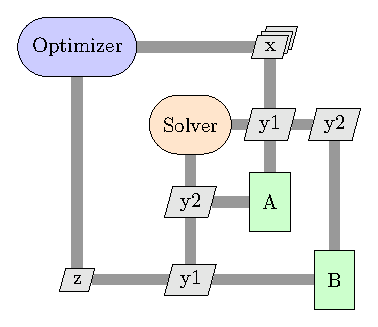
\includegraphics[width=0.4\textwidth]{xdsm/mdf_sample}
        \caption{Notional design problem with MDF problem formulation}
        \label{fig:MDF:XDSM}
    \end{figure}

    In Fig. \ref{fig:MDF:XDSM}, the optimizer varies the design variable $A.x$, a large vector.
    The solver converges variables $y_1$ and $y_2$ from disciplines $A$ and $B$. Applying a
    Newton-based method requires $\frac{\partial A.y_1}{\partial A.y_2}$ and $\frac{\partial B.y_2}{\partial B.y_1}$
    to converge, but $\frac{\partial A.y_1}{\partial A.x}$ is not relevant. By using the linear operator derivatives method,
    the cost of multiplying by $\frac{\partial A.y_1}{\partial A.x}$ can be avoided while converging the solver and only
    computed as part of the outer optimization loop.

    \section{Small Satellite Design Problem}

    Cubesat investigating Atmospheric Density Response to Extreme driving (CADRE)
    is a mission funded by the National Science Foundation to study the
    response of the thermosphere to auroral phenomena\cite{cutler2011cubesat}.
    The small satellite design problem optimizes the design of a cubesat for the CADRE mission.
    This problem was originally implemented and solved by Hwang et al.\cite{CADRE2012} using
    Martins and Hwang's matrix-free gradient strategy. The analysis models the orbit of a cubesat
    as it performs a mission over the course of 1 year. The full mission is represented
    by 6 half-days of operation, computed at conditions 1, 3, 5, 7, 9, and 11 months after launch.

    \begin{table}
        \centering
        \caption{Small satellite design problem formulation}
        \begin{tabular}{r l l l}
            \toprule
            & Variable/Function & Description & Quantity \\
            \midrule
            maximize            & $\sum_{i=1}^6 D_i$ & Data downloaded \\
            \\
            with respect to & $0 \le I_\text{setpt} \le 0.4$ & Solar panel current & $300 \times 12 \times 6$ \\
                                    & $0 \le \gamma \le \pi / 2$ & Roll-angle profile & $300 \times 6$ \\
                                    & $0 \le P_\text{comm} \le 25$ & Communication power & $300 \times 6$ \\
                                    & $0 \le \text{cellInstd} \le 1$ & Cell vs. radiator & $84$ \\
                                    & $0 \le \text{finAngle} \le \pi / 2$ & Fin angle & $1$ \\
                                    & $0 \le \text{antAngle} \le \pi$ & Antenna angle & $1$ \\
                                    & $0.2 \le iSOC \le 1$ & Initial state of charge & $6$ \\
                                    & & Total & $25292$ \\
            \\
            subject to          & $I_\text{bat} - 5 \le 0$ & Battery charge constraint & $6$ \\
                                    & $-10 - I_\text{bat} \le 0$ & Battery discharge constraint & $6$ \\
                                    & $0.2 - SOC \le 0$ & Battery capacity constraint & $6$ \\
                                    & $SOC - 1 \le 0$ & Battery capacity constraint & $6$ \\
                                    & $fSOC - iSOC = 0$ & SOC periodicity constraint & $6$ \\
                                    & & Total & $30$ \\
            \bottomrule
        \end{tabular}

        \label{eqn:cadre_formulation}
    \end{table}

    The objective of the optimization was to maximize the total amount of data transmitted to the ground
    station over these six design points. In their original work, Hwang et. al. located the ground station 
    for receiving data in Ann Arbor, Michigan. Because the satellite was launched into a polar orbit moving the ground station 
    closer to one of the polls would increase the amount of data collected. McMurdo Station, 
    Antarctica is located very close to the South Poll and is an existing scientific research facility. 
    So for this work, the McMurdo was selected as the ground station location. 

    There were seven design variables listed in Tab.~\ref{eqn:cadre_formulation}.
    Three of them, $\gamma$, $I_{setpt}$, and $P_{comm}$, were arrays of time-varying schedules for the attitude,
    solar panel current, and communications power, respectively. The remaining four, $cellInstd$, $finAngle$, $antAngle$, and $iSOC$,
    were all physical design variables of the satellite. All together there are 25,292 design variables.
    The five constraints for the problem relate to the battery charge rate, battery discharge rate,
    minimum battery capacity, maximum battery capacity, and a battery state-of-charge (SOC) periodicity
    constraint. Each constraint was a length 6 vector with a value representing each of the 6 different
    orbits, yielding a total of 30 constraints. Since the problem has significantly more design
    variables than it does objectives and constraints, it was solved using adjoint gradients.


    \begin{figure}[!htbp]
        \centering
        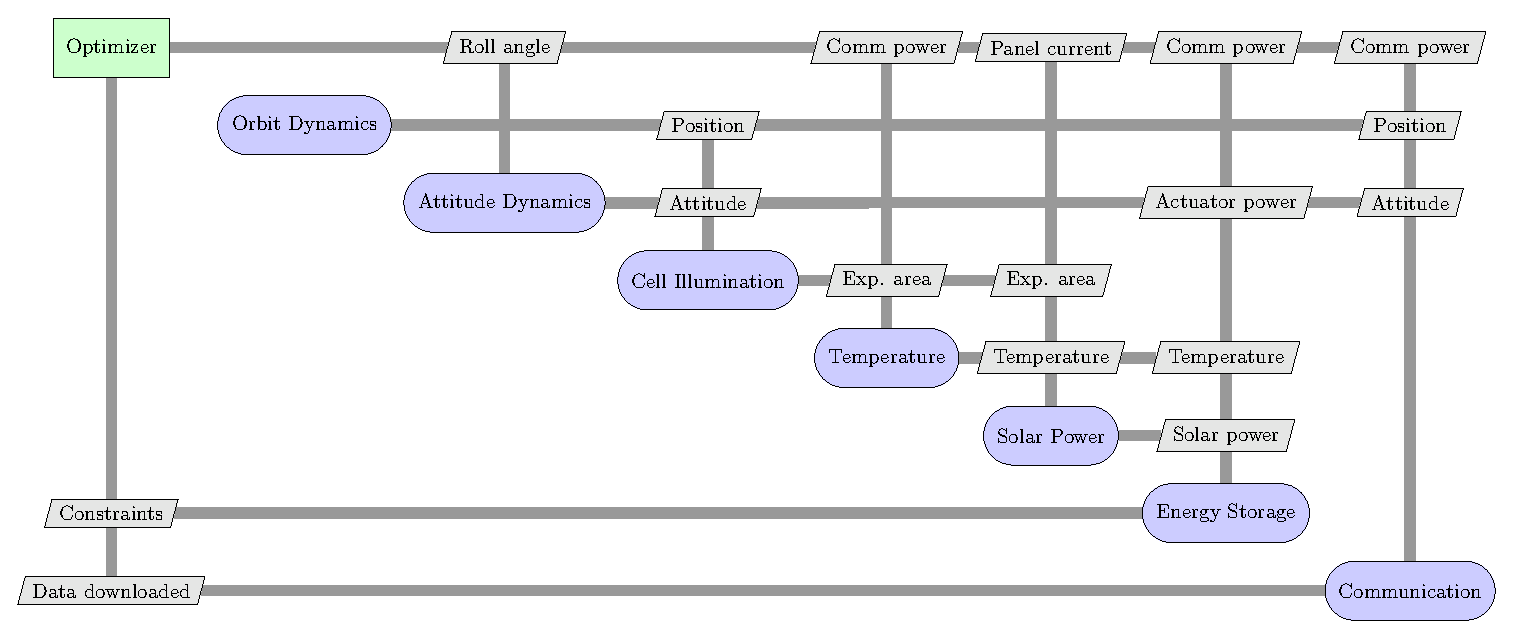
\includegraphics[width=0.95\textwidth]{xdsm/cadre_xdsm}
        \caption{Extended Design Structure Matrix (XDSM) showing the structure of the small satellite design problem}
        \label{fig:cadre_xdsm}
    \end{figure}

    Overall, the problem can be broken down into seven distinct disciplines: orbit dynamics, attitude dynamics, cell illumination,
    temperature, solar power, energy storage, and communication. Figure \ref{fig:cadre_xdsm} shows how each of the disciplines
    relate to each other in the optimization problem. The actual implementation of the problem further
    subdivided most of the disciplines into smaller subdisciplines. The true component-level dependency
    graph, given in Fig. \ref{fig:cadre_graph}, has 39 different components. The full graph, including all variable and
    subvariable nodes, is omitted for visual clarity.

    From a problem structure standpoint, this problem has three significant features. First, the large number of
    disciplines, design variables, and the complex connections between them make assembling the linear system to solve for gradients
    challenging to do by hand. Second, although the problem does not have any explicit interdisciplinary coupling,
    there is coupling from the SOC periodicity constraint, $fSOC - iSOC = 0$, which is dependent on many of the
    disciplines. Third, all disciplines were implemented with analytic derivatives so that no finite differencing was
    necessary.

    \begin{figure}[!htb]\begin{center}
      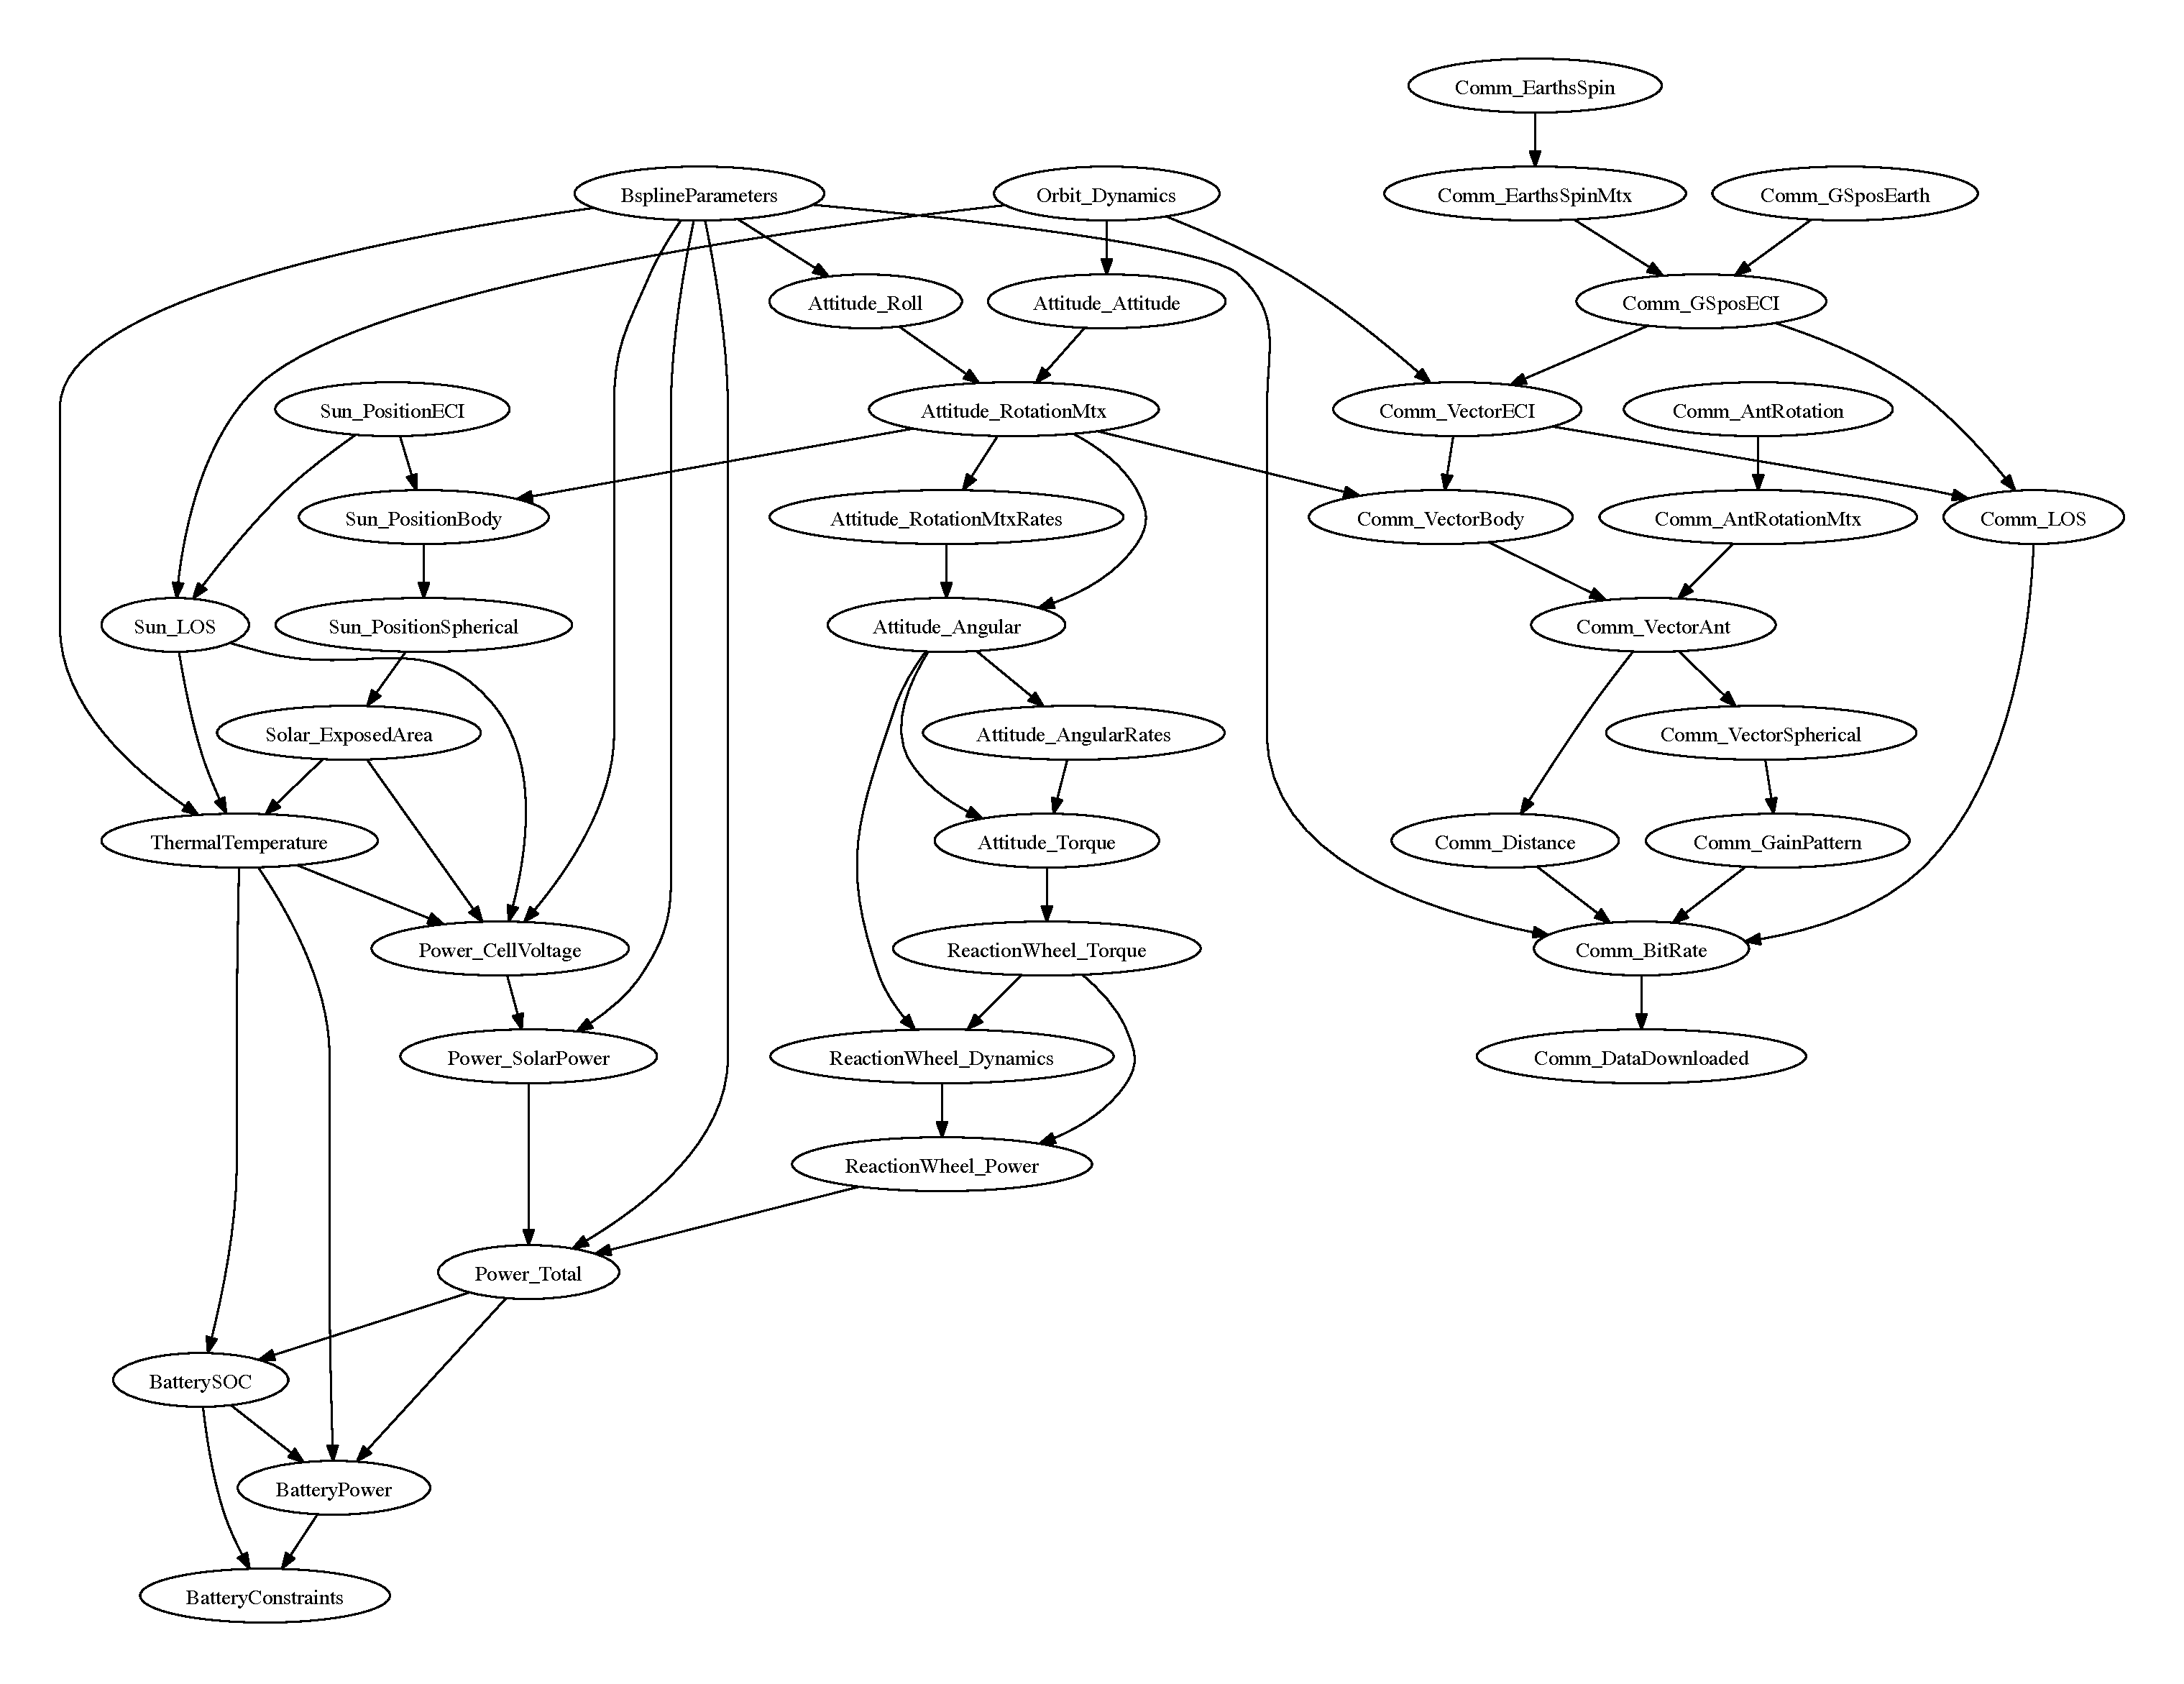
\includegraphics[width=.95\textwidth]{images/CADRE.pdf}
      \caption{ Dependency graph for the satellite problem. \label{fig:cadre_graph}}
    \end{center}\end{figure}

    \subsection{Optimization Results}

        The final optimal design yielded 1000 GibaBytes (GB) total data downloaded over the 6 time points considered. 
        Figure \ref{fig:trajectories} shows ground trace for the satellite colored by communications bit rate
        for all 6 time points combined. Bit rate can be compared directly with the communications power in
        Fig. \ref{cadre_data_results}, where large spikes in communications bit rate correspond to passes over the ground station requiring 
        power to the communication system for transmission. Figure \ref{cadre_data_results} shows key design and performance data 
        for the design problem over the course of the optimization for all six points in time considered. Data is shown for the 
        initial condition, at 50 function evaluations, and for the final optimum solution. At the initial condition
        the roll angle is a constant 45 degrees, the communication power is uniformly 0, and battery state of charge drops quickly below 0. 
        This design is obviously terrible and indicates clearly why the optimizer had to work hard to find a feasible solution. 
        By the 50th function evaluation, the optimizer found a sinusoidal pattern in the roll angle and a saw-tooth pattern 
        for SOC. The roll angle pattern allowed the satellite to continually pitch toward the sun throughout its orbits. 
        The SOC exhibited sharp drops whenever a communications opportunity arose and the power to the communication system was ramped up. 
        The data from the final optimized design shows a refinement of the direction already discussed with a much stronger convergence for 
        all the constraints. 

        \begin{figure}[!htb]
            \centering
            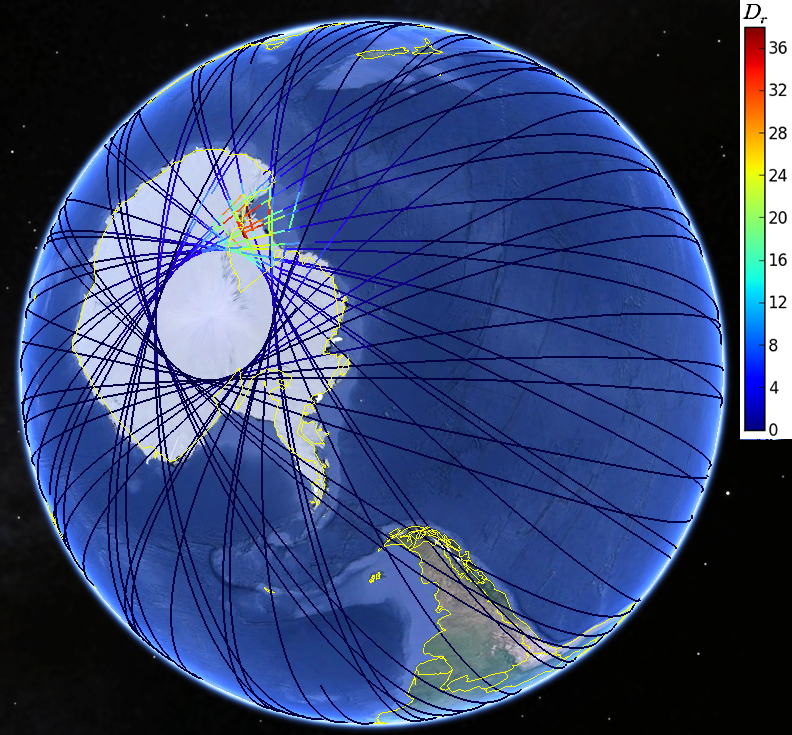
\includegraphics[width=0.49\textwidth]{images/allpts_gearth_mcmurdo}
            \caption{Ground trace of the satellite trajectories 
            for all the design points colored by communications bit rate. 
            \label{fig:trajectories}
            }
        \end{figure}


        \begin{figure}[!htb]
          \centering
          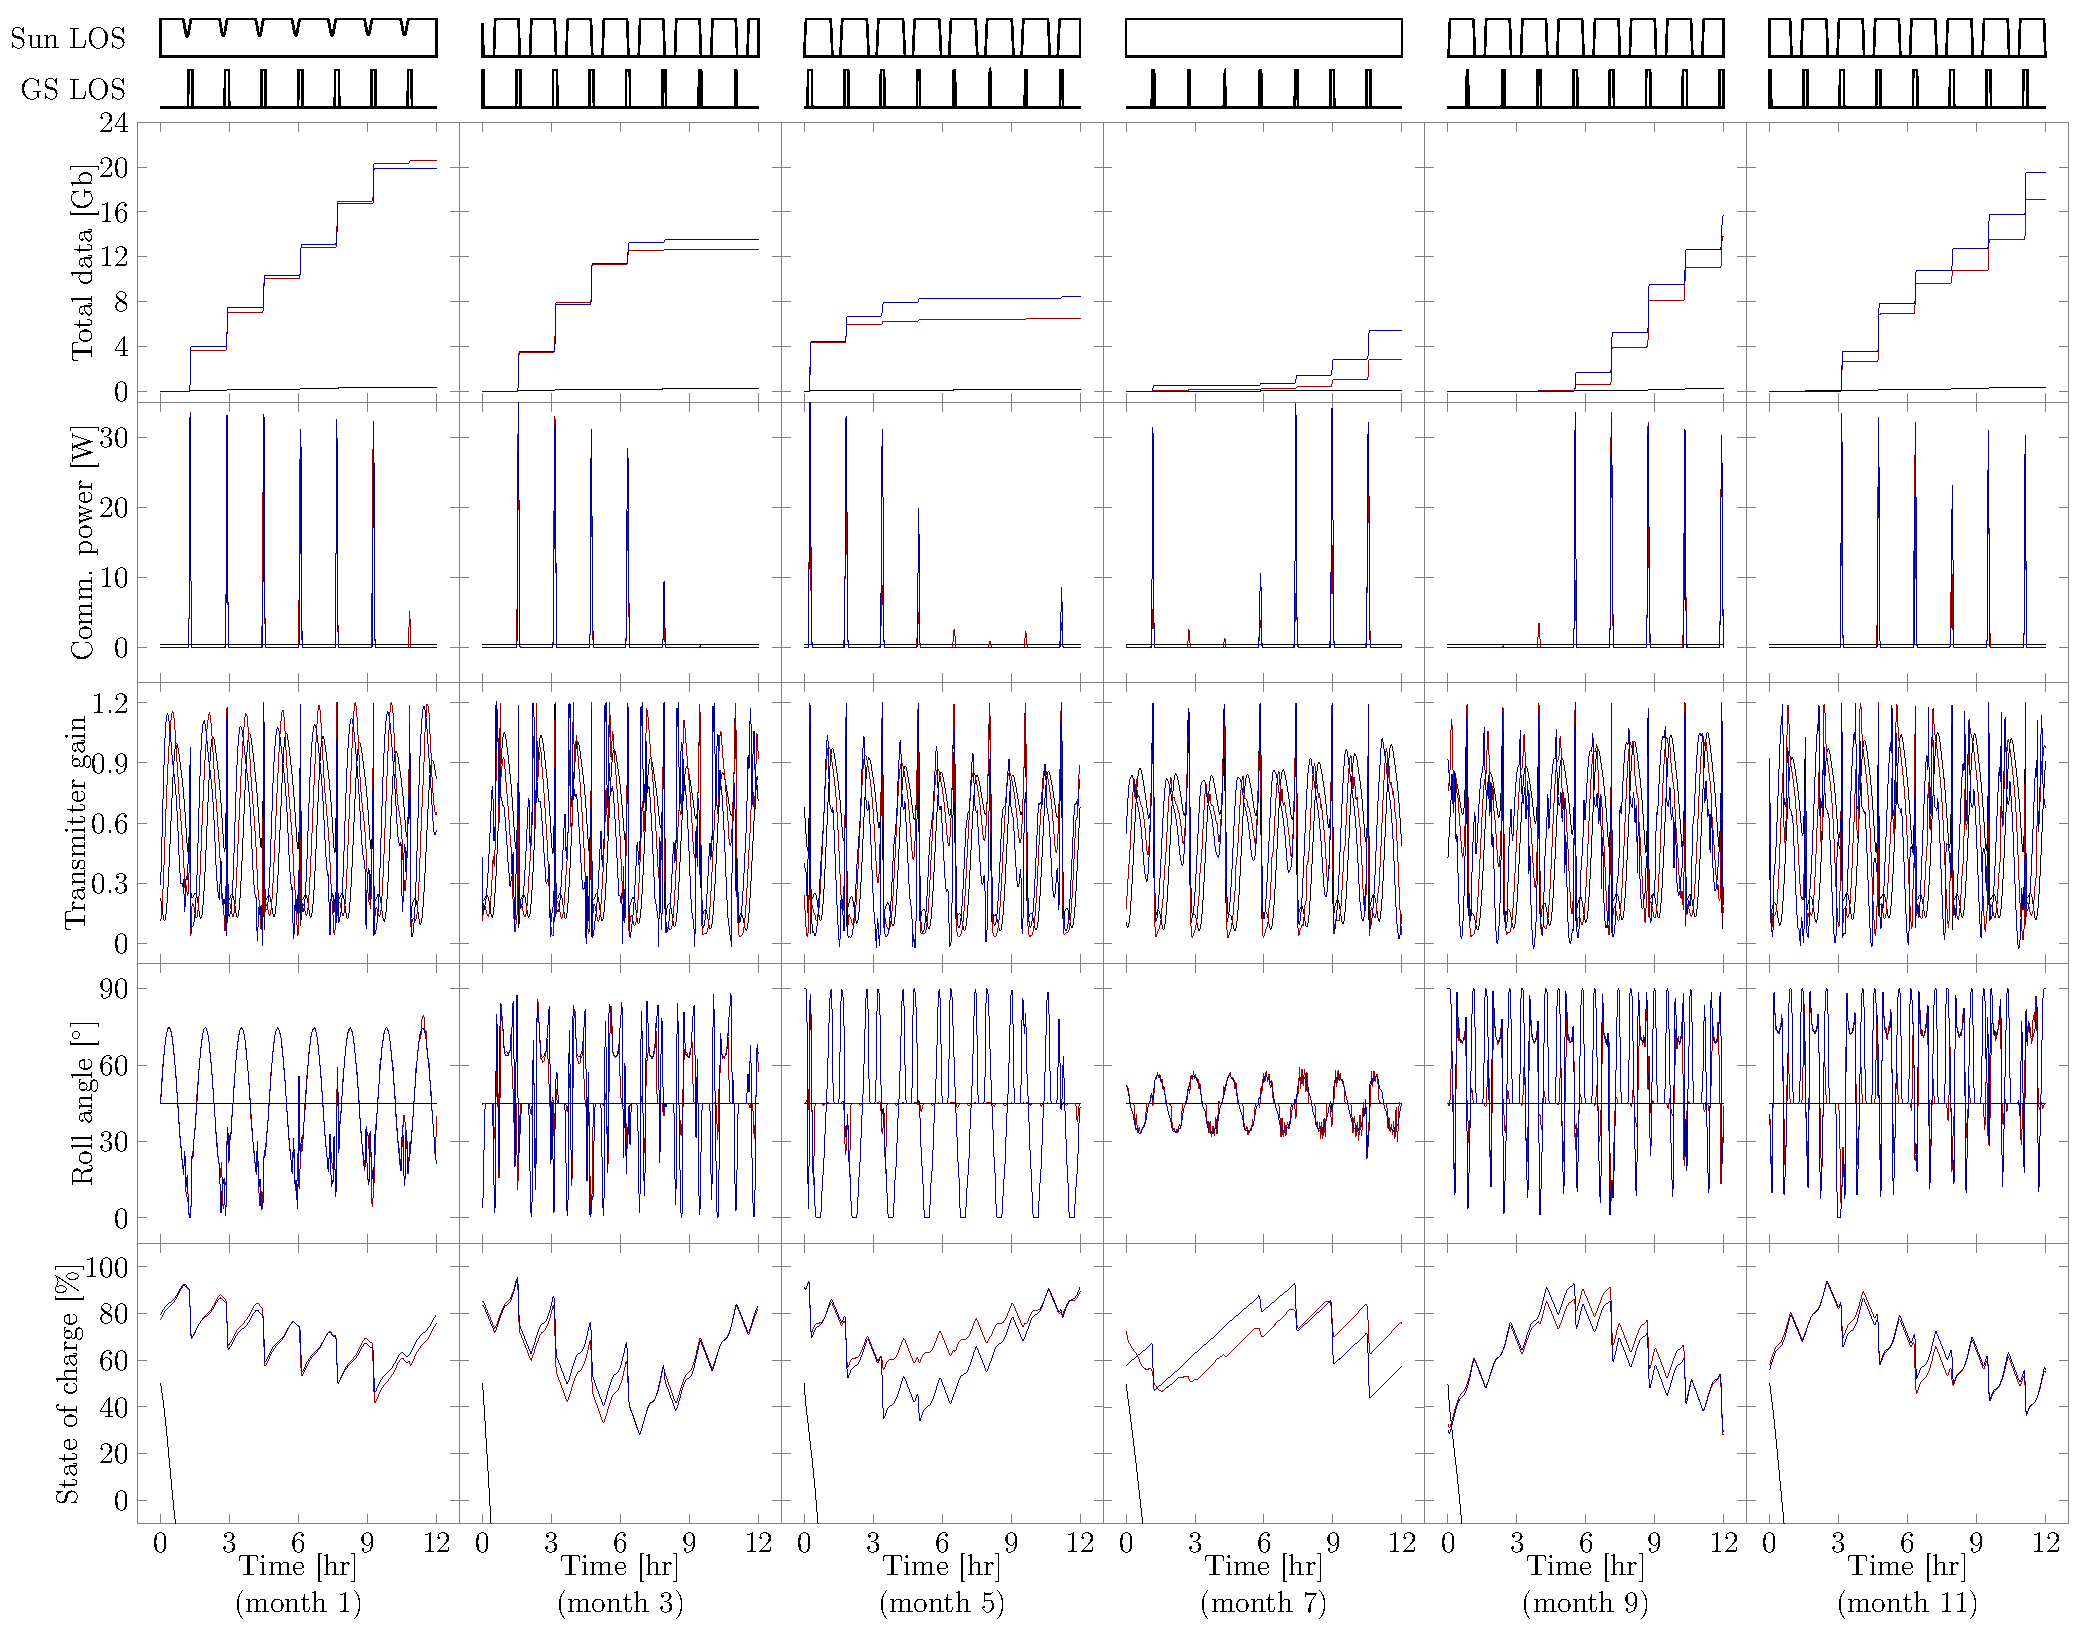
\includegraphics[width=\textwidth]{images/cadre_data}
          \caption[width=0.4\textwidth]{Plots of the SOC, roll angle, transmitter gain, communications power, and total data downloaded for 
          each of the 6 time periods analyzed. Data is presented for the initial condition (black), at 50 function evaluations (red), and at the final 
          optimal point (blue). 
          \label{cadre_data_results}
          }
        \end{figure}


        Roll angle data in Figure \ref{cadre_data_results} roughly approximates a sine function
        with a period of 90 minutes (the approximate orbital period of the satellite), with short-term perturbations during the time
        periods where line of sight is gained with the ground station. That is, the optimizer
        converged to a solution with the satellite continuously turned to maximize exposure to the sun,
        except when turning to point its antenna towards the ground station. This dynamic is also reflected in the SOC
        data plotting in the bottom row, with the battery losing charge quickly during
        communication with the ground station but recharging while tracking with the sun.



        \clearpage
        

        \subsection{Performance Results}

            The OpenMDAO implementation of the satellite problem was executed on a
            Macbook Pro (2.6 GHz Core i7 processor, 16GB 1600 MHz DDR3 memory, running OSX 10.8.5).
            The problem was converged to a termination tolerance of $10^{-4}$ using the SNOPT\cite{gill2005snopt} optimizer. 
            The problem was run twice, once with a graph full problem graph including all variables regardless of relevance 
            and a second where the graph was reduced based on the algorithms discussed in Section \ref{sec:determing relevance}. 
            The effects of the graph reduction are shown in Table \ref{tab:cadre-relevance-reduction}. The number of variables in
            the graph, and hence the size of the linear system that needs to be solved, was reduced by 18\%. This reduction 
            yielded a drop in runtime of about 16\%. 


            \begin{table}
                \centering
                \caption{Effects of relevance-based problem reduction on derivatives linear system size}
                  \begin{tabular}{l c c c}
                      \toprule
                                   & Full Graph & Reduced Graph & \% Reduction\\
                      \midrule
                      \# Variables  & 2.15e6 & 1.76e6 & 18\%\\ 
                      \# Components & 39 & 29 & 25.6\%\\ 
                      Derivative Solve Time (sec) & 126 & 87 & 31\%\\ 
                      Total Run Time (hours) & 10.68 & 8.94 & 16.3\%\\ 
                      \bottomrule
                  \end{tabular}    
                \label{tab:cadre-relevance-reduction}
            \end{table}


            \begin{figure}[!htb]
            \centering
            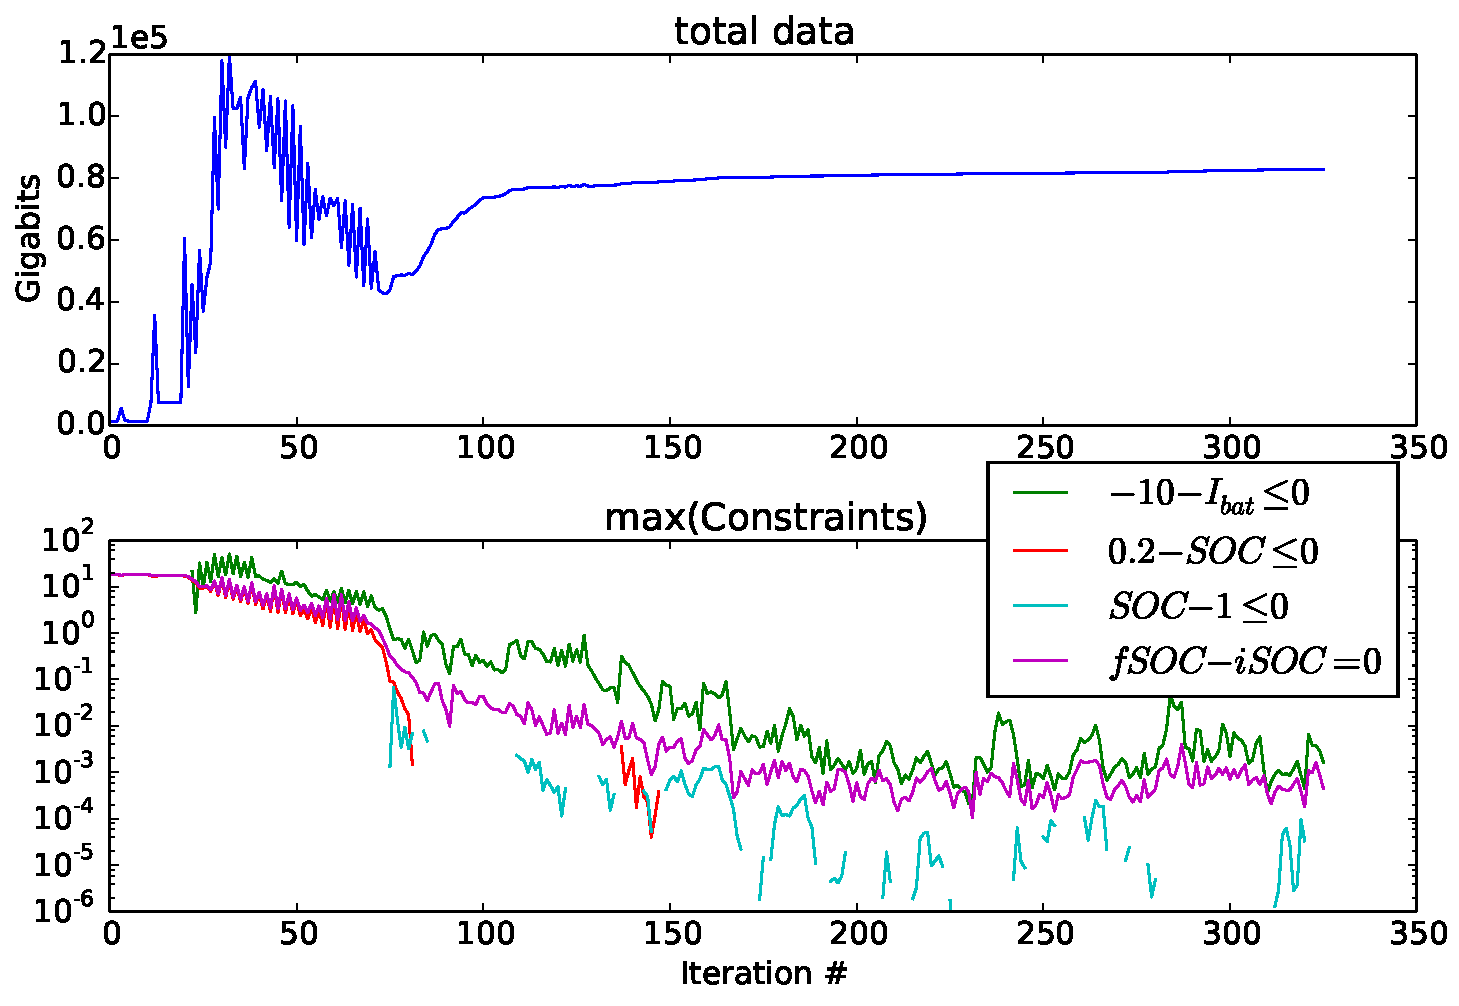
\includegraphics[width=0.99\textwidth]{images/cadre_opt_progress}
            \caption[width=0.22\textwidth]{Iteration history of the satellite problem.
            \label{convergence}
            }
            \end{figure}

          
            Figure \ref{convergence} compares function evaluation history over the course of
            the optimization between the full and reduced graph cases. The top plot shows the value of the objective function, the total data downloaded.
            The bottom plot shows the 2-norm of the constraints. In both cases the objective function oscillated greatly early in the optimization while 
            the optimizer sought a feasible solution. The saw-tooth pattern in the results occurs when the optimizer performs large
            jumps during a line search. When the line search moves too far, the objective and convergence can both get worse, causing the 
            optimizer to back to recover. Around the 100th iteration a mostly feasible solution was found and
            the remaining effort was spent improving the objective.

            \begin{table}
              \centering
              \caption{Comparison between the full and reduced problem graphs for different-sized small satellite design problems}
                \begin{tabular}{c c c}
                    \toprule
                    Full Graph & Reduced Graph & Reduction\\
                    \midrule
                    1.08e6 & 8.8e5 &  18\%\\
                    2.15e6 & 1.76e6 & 18\%\\
                    4.30e6 & 3.52e6 & 18\%\\
                    8.60e6 & 7.05e6 & 18\%\\
                    1.72e7 & 1.41e7 & 18\%\\
                    \bottomrule
                \end{tabular}
                \label{tab:cadre-problem-sizes}
            \end{table}


            \begin{figure}[!htbp]
                \centering
                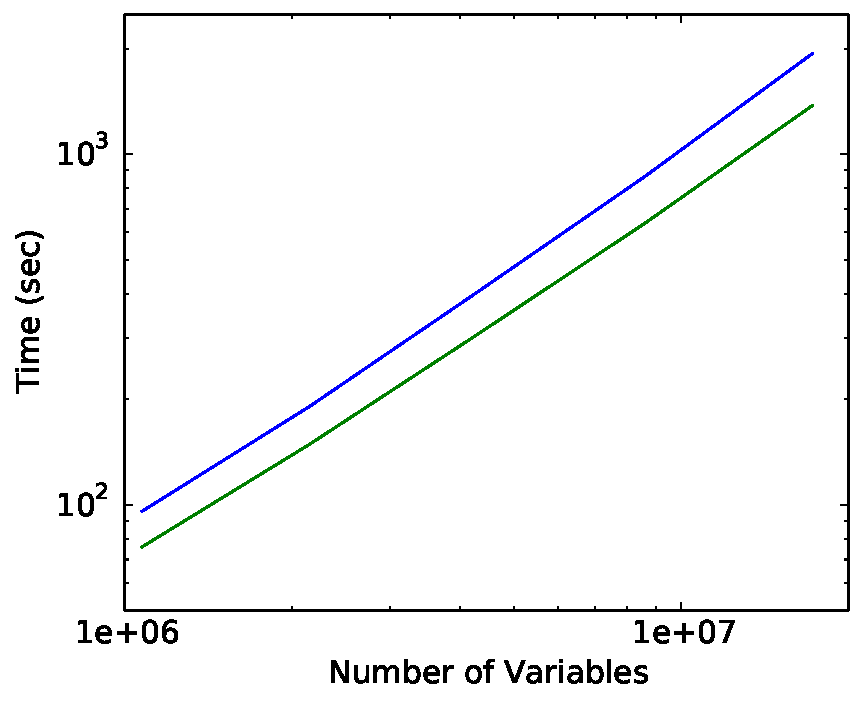
\includegraphics[width=0.5\textwidth]{images/cadre_var_scaling}
                \caption{Adjoint solution cost as a function of number of variables in the problem formulation.}
                \label{fig:cadre-compute-cost}
            \end{figure}

            Although the overall reduction in optimization cost was 16\%, reduction of dependency graph provided
            a 30\% reduction in the cost to compute adjoint derivatives. 
            Figure \ref{fig:cadre-compute-cost} shows a log-log plot of computational cost for 31 adjoint solves (30 constraints + 1 objective) versus the
            number of variables in the full problem. The trend shows linear growth for both the full and reduced
            versions of the graph, with a constant ratio between them. This problem was scaled by
            refining the time discretization for the integration of ordinary differential equations. Although
            increasing the amount of time steps taken does increase the sparsity of the individual discipline Jacobians,
            it does not have an impact on the sparsity of the problem formulation. In other words, although the size of the
            variable arrays grows, the structure of the dependency graph remains constant. Table \ref{tab:cadre-problem-sizes}
            demonstrates the consequences of the constant problem formulation sparsity, which yields a fixed ratio between
            the full and reduced problem size.

            The 30\% reduction in computational cost for solving the gradients did not directly translate into
            equivalent savings in the overall optimization cost because of the by the nontrivial cost of
            SNOPT itself. This problem requires a large number of minor iterations, where SNOPT solves a quadratic subproblem.
            The cost of solving these subproblems is not affected by the cost of computing the derivatives and hence
            reduces the overall computational savings. This characteristic will be highly problem-dependent, and is not expected
            to be so significant for all problems. Also, the overhead from the optimizer would get less significant as the 
            computational cost of the analyses and derivative solves increased. Thus, the efficiency gain from the graph reduction 
            would be more significant for larger, more expensive problems.


  \section{Wind Turbine Design Problem}

    The goal of this design problem was to optimize a horizontal-axis wind turbine to minimize
    the cost of energy at a land-based site. The problem includes the design of the rotor blades
    with a coupled aero-structural analysis as well as the structural design of the hub, nacelle,
    and tower.  Cost models for the turbine and wind plant are included
    to assess trade-offs in energy capture and capital and operational costs.  The analyses
    for this model are part of the Wind-Plant Integrated Systems Design \& Engineering Model (WISDEM)
    developed at the National Renewable Energy Laboratory (NREL) as part of a larger effort
    to develop a physics- and cost-based design optimization framework for wind turbines  \cite{Dykes2014a,Ning2013a,Ning2014,Ning2014d}.

    Wind turbine design involves a large number of structural constraints specified by various standards.  This optimization problem utilizes a subset of the design requirements specified by the International Electrotechnical Commission for land-based designs \cite{IEC}.  Structural considerations include maximum deflections, stress and strain limits, resonance, buckling, and manufacturing considerations.   A typical problem formulation is given in Tab.~\ref{tab:coe_formulation}.  Bound constraints were chosen to be large enough to not be active, except for those that must be restricted because of manufacturing or transportation reasons.  For simplicity, safety factors are not included in the list of constraints.

    \begin{table}[!htb]
        \centering
        \caption{Horizontal-axis wind turbine optimization problem description}
        \begin{tabular}{r l l l}
            \toprule
            & Variable/function & Description & Quantity \\
            \midrule
            minimize            & $COE$ & Cost of energy \\
            \\
            with respect to & $0.4 \le c \le 20$ & Chord distribution & $5$ \\
                                    & $-10 \le \theta \le 30$ & Twist distribution & $4$ \\
                                    & $0.005 \le t_{sc} \le 0.2$ & Spar-cap thickness distribution & $5$ \\
                                    & $0.005 \le t_{te} \le 0.2$ & Trailing-edge panel distribution & $5$ \\
                                    & $3 \le \lambda \le 14$ & Tip-speed ratio in Region 2 & $1$ \\
                                    & $40 \le L_{blade} \le 100$ & Blade length & $1$ \\
                                    & $0.1 \le L_{shaft} \le 10$ & Low-speed-shaft lengths & $2$ \\
                                    & $0.01 \le h_{beam} \le 10$ & Bedplate I-beam sizing & $2$ \\
                                    & $3.87 \le d \le 20$ & Tower diameter & $3$ \\
                                    & $0.005 \le t \le 0.2$ & Tower wall thickness & $3$ \\
                                    & $0.25 \le z_{waist} \le 0.75$ & Tower waist location & $1$ \\
                                    & $50 \le H \le 200$ & Tower height & $1$ \\
                                    & & Total & $33$ \\

            \\
            subject to          & $\delta_{tip} \le \delta_{max}$ & Blade tower strike & $1$ \\
                                    & $\delta_{ground} \ge \delta_{min}$ & Blade ground clearance & $1$ \\
                                    & $\epsilon \le \epsilon_{ult}$ & Ultimate strain in blades & $24$ \\
                                    & $\epsilon \le \epsilon_{cr}$ & Panel buckling in blades & $14$ \\
                                    & $\delta_{lss} \le \delta_{max}$ & Deflection limits in low-speed shaft & $4$ \\
                                    & $\delta_{bdp} \le \delta_{max}$ & Deflection limits in bedplate & $2$ \\
                                    & $\sigma_{bdp} \le \sigma_{ult}$ & Ultimate stress in bedplate & $2$ \\
                                    & $\sigma_{twr} \le \sigma_{ult}$ & Ultimate stress in tower & $14$ \\
                                    & $\sigma_{twr} \le \sigma_{shell}$ & Shell buckling in tower & $14$ \\
                                    & $\sigma_{twr} \le \sigma_{global}$ & Global buckling in tower & $14$ \\
                                    & $f \ge \Omega_{rotor}$ & Tower resonance avoidance & $1$ \\
                                    & $d/t \ge 120$ & Weldability & $1$ \\
                                    & $d_{top}/d_{base} > 0.4$ & Manufacturability & $1$ \\
                                    & & Total & $93$ \\
            \bottomrule
        \end{tabular}
        \label{tab:coe_formulation}
    \end{table}


    There are 33 design variables, 1 objective, and 93 constraints. An additional maximum tip-speed constraint of
    80 m/s is imposed directly in the analysis.  Because there are
    fewer design variables than quantities of interest, the problem was solved with
    forward derivatives. In addition, the relatively small size of the design space
    enabled a comparison between the use of analytic and finite-difference gradients. There were 10 disciplines
    involved in the top level of the model, as seen in Fig.~\ref{fig:xdsm_wt}.  Half of these disciplines represented the physics of the problem, aerodynamic and structural models of the turbine components, while the other half encapsulated the various cost components.  The aero-structural coupling was achieved through a fixed point iteration around the rotor discipline, converging the deflected blade shape to a tolerance of $1\times10^{-8}$. OpenMDAO automatically computes the coupled derivatives around this convergence loop.


    \begin{figure}[!p]
        \centering
        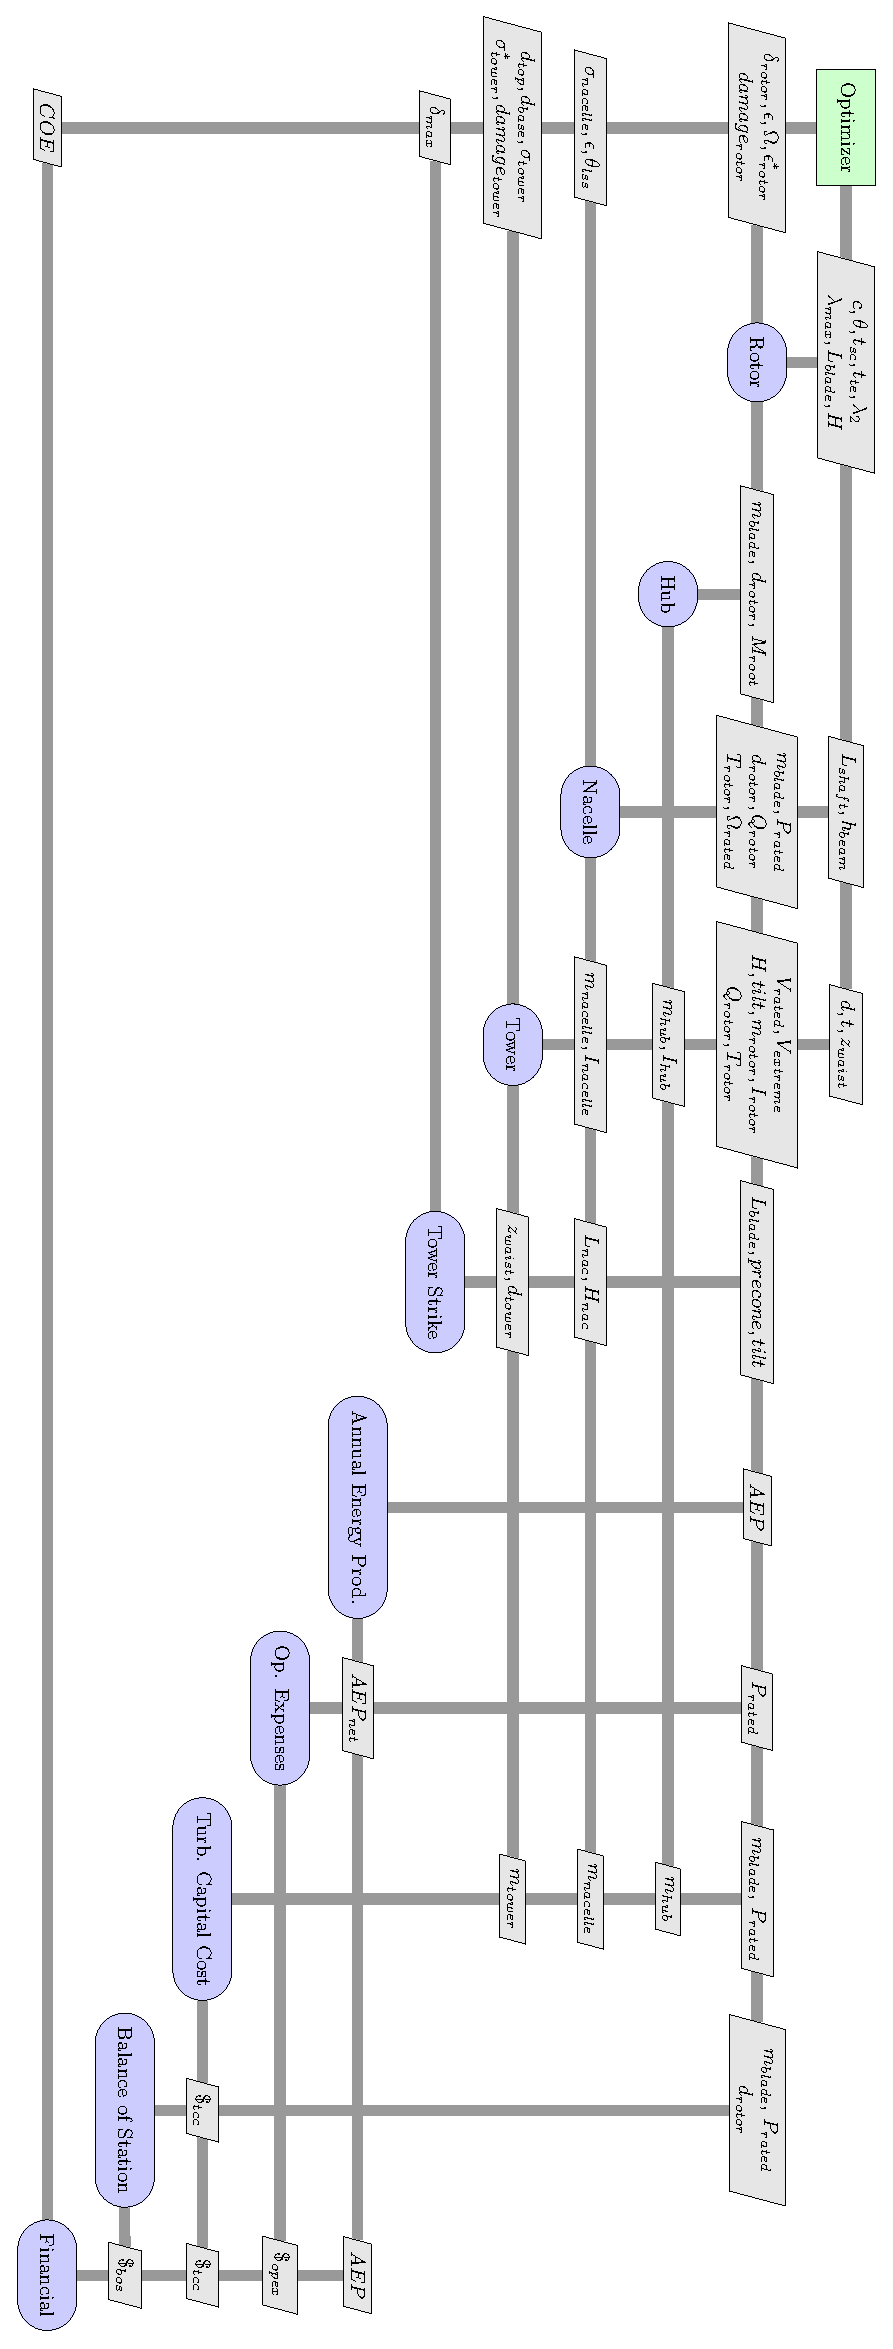
\includegraphics[height=\textheight]{xdsm/wt_xdsm}
        \caption{XDSM diagram of the top level wind turbine design optimization problem}
        \label{fig:xdsm_wt}
    \end{figure}

    Similar to the small satellite design problem, many of the disciplines were further
    subdivided into more than one component for implementation. In the
    satellite problem, all components were left at the same level in the model, but for this problem
    actual subassemblies of components were made (e.g., Rotor, Hub, Nacelle, Tower, Turbine Capital Cost,
    and Balance of Station). This highly nested structure was designed to provide modularity,
    to allow a wide range of researchers to build discipline models that can be swapped in and out.
    It also greatly simplifies the complexity of the top level model.
    The presence of these subassemblies is relevant to how the derivatives are computed.
    They are treated as single discipline components from the perspective of the top level model,
    meaning that when derivatives are requested from the assembly, it will internally solve
    for its own boundary derivatives and report them to the top level assembly. Table \ref{tab:wt_comp_counts}
    summarizes number of subassemblies and components in those subassemblies for the overall model. There 
    are a total of 104 components spread out between 22 different subassemblies. 

    \begin{table}\centering
      \caption{Component and subassembly counts for the wind turbine design problem at different levels of 
      the model}
      \label{tab:wt_comp_counts}
      \begin{tabular}{l c c}
      \toprule
             & \# Components & \# Subsssemblies \\
      \midrule
      Top level & 1 & 9\\
      \ \  Rotor & 33 & 0\\
      \ \  Hub & 4 & 0\\
      \ \  Nacelle & 10 & 0 \\
      \ \  Tower & 16 & 0\\
      \ \ Tower Strike & 1 & 0 \\
      \ \  Annual Energy Production & 1 & 0 \\
      \ \  Turbine Capital Cost & 1 & 3  \\
      \ \ \ \ Nacelle Capital Cost & 8 & 0  \\
      \ \ \ \ Tower Capital Cost & 2 & 0 \\
      \ \ \ \ Rotor Capital Cost & 6 & 0  \\
      \ \  Operational Expenses & 1 & 0  \\
      \ \  Balance of Station & 19 & 0 \\
      \ \  Financial & 1 & 0 \\ 
      \hline
      Total & 104 & 12 \\

      \bottomrule
      \end{tabular}
    \end{table}


    \begin{figure}[!htbp]
        \centering
        %[Insert subassembly Dependency Graphs]
        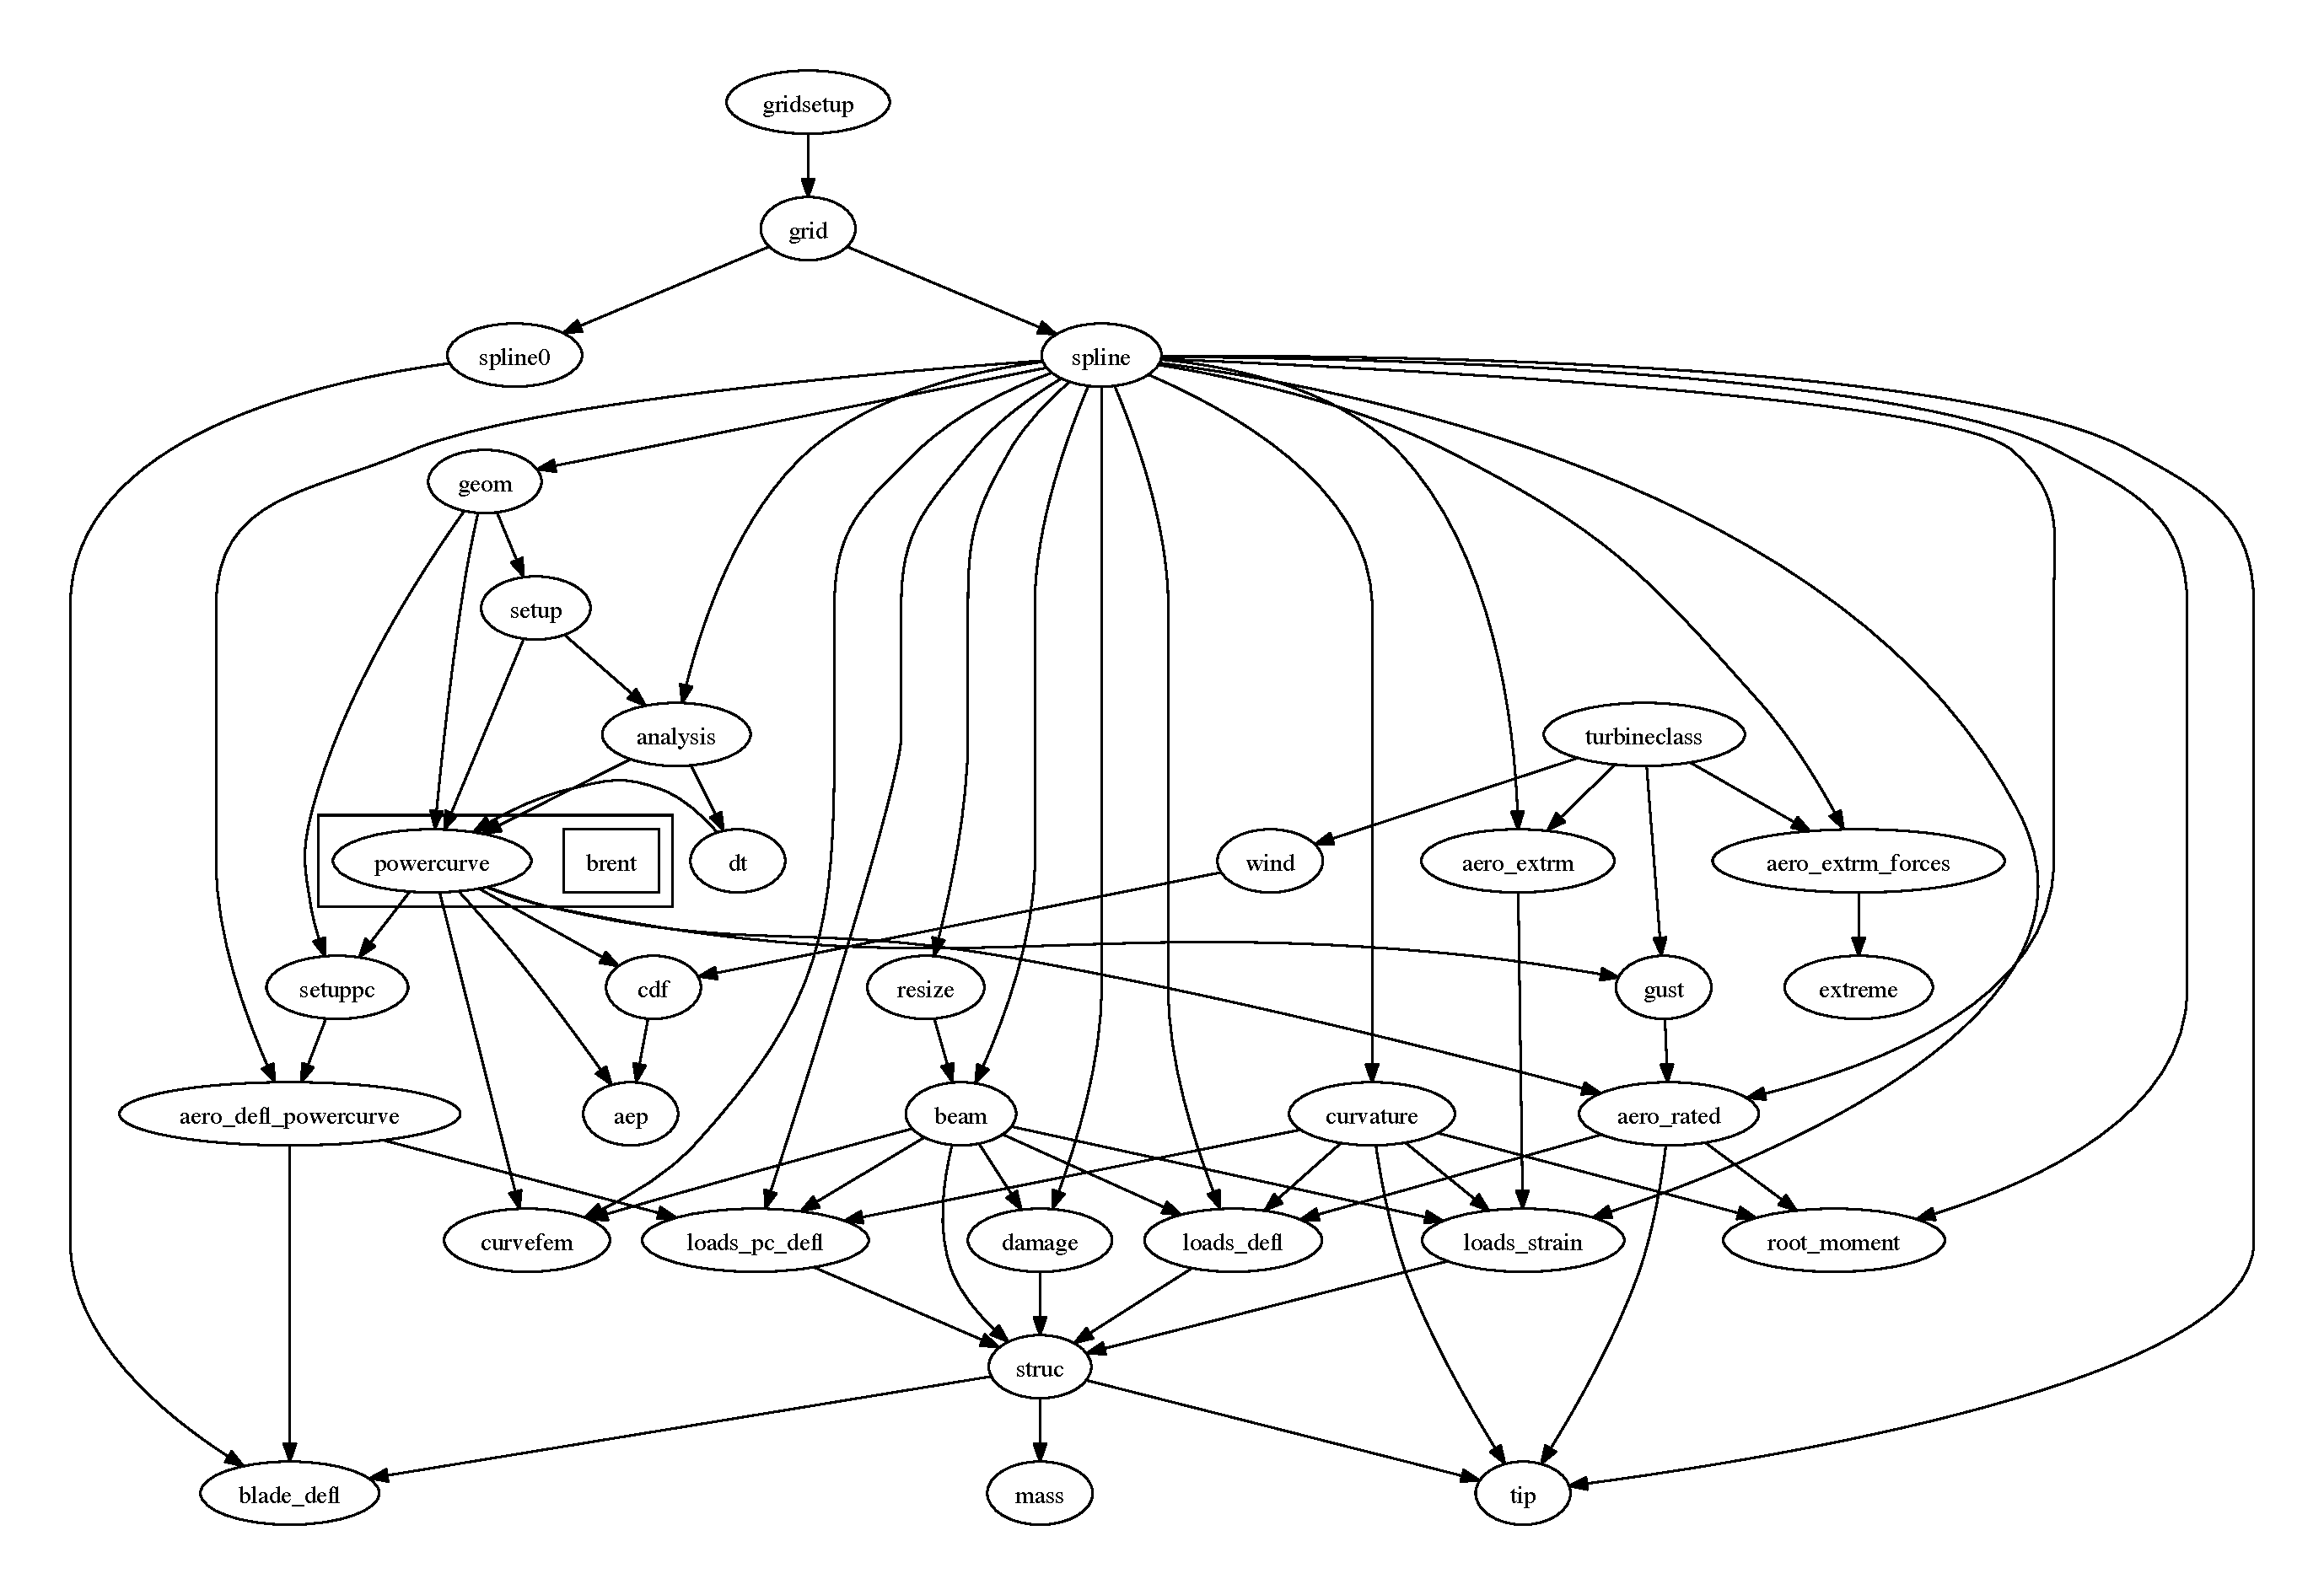
\includegraphics[width=0.95\textwidth]{images/rotor_depgraph}
        \caption{Rotor subassembly dependency graph}
        \label{fig:wt_sub_depgraph}
    \end{figure}

    The Rotor discipline in particular has an important internal feature with regard to computing derivatives.
    The rotor subassembly is responsible for modeling aerodynamics, using CCBlade\cite{NING:BEM},
    a blade element momentum (BEM) tool specifically tailored to optimization. It includes
    an internal convergence on the PowerCurve discipline, with a Brent solver \cite{Brent1971}, to find the
    rated speed, $V_{rated}$, for the wind turbine. This convergence loop requires the Rotor
    subassembly to compute coupled derivatives. Figure \ref{fig:wt_sub_depgraph} shows the complete
    dependency graph for just the Rotor discipline, which has 33 components in total.  The internal solver used to 
    find rated speed is highlighted with a box in the figure.

    The structures discipline for the blades was modeled with pBEAM \cite{Ning2013b},
    a beam finite element code, PreComp \cite{Bir2005}, a structural property tool for
    composite blades, and additional structural modules for panel buckling and fatigue. In the Tower subassembly,
    aerodynamics was modeled with power-law wind profiles and cylinder drag theory.
    Tower structures was modeled with pBEAM and additional modules for shell buckling,
    global buckling, and fatigue.  Some drivetrain components were modeled with scaling
    relationships (bearings, yaw system, generator), while others used bottom-up physics
    models (bedplate, gearbox, low-speed shaft).

    Analytic gradients were derived for all aerodynamic components, cost components, and many of the 
    structural components using a mixture of hand-derivation and automatic differentiation.  Some of 
    the remaining structural components (pBEAM and PreComp) did not yet provide analytic gradients.  
    For these components, the output was still continuously differentiable, and their Jacobians were 
    estimated with finite differencing.  This led to a mixed derivative scenario where analytic 
    Jacobians and the finite difference Jacobians were used together to solve for system-level 
    derivatives.


    % \begin{figure}[!htbp]
    %     \centering
    %     %Insert Top Level Dependency Graph]
    %     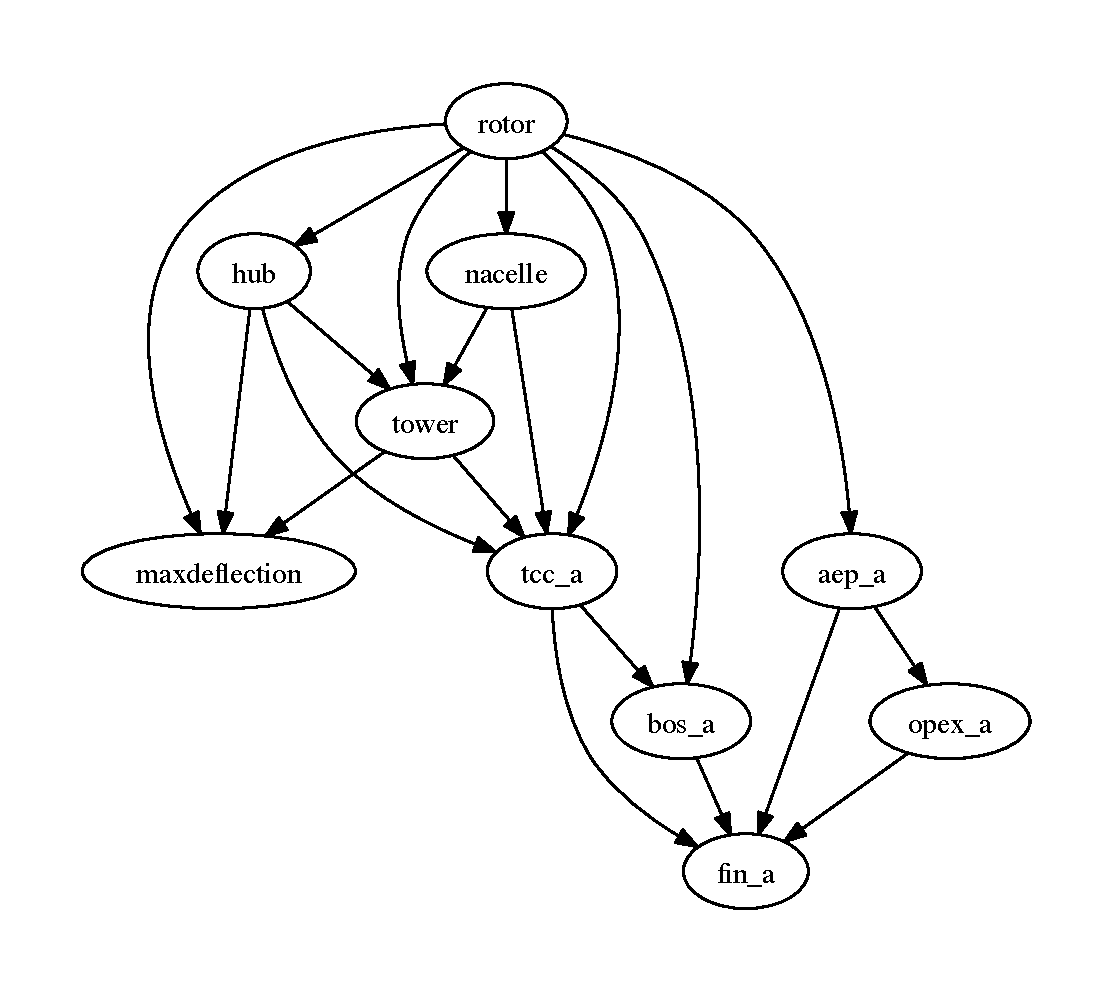
\includegraphics[width=0.5\textwidth]{images/wt_depgraph}
    %     \caption{Wind turbine problem top level dependency graph}
    %     \label{fig:wt_top_depgraph}
    % \end{figure}

    % \clearpage


    This problem has one additional interesting characteristic in its
    problem formulation: a number of data connections throughout the dependency
    graph are never relevant to the derivatives calculations. These nonrelevant
    variables are used for various settings and initialization values throughout the
    model, such as the number of blades on the rotor or the density of air. For convenience
    and consistency, the variables do still have connections so that the right values can
    be set in one place and passed to all necessary components automatically.
    Such variables, especially when they are integers (or otherwise nondifferentiable)
    necessitate the graph-based approach to identify irrelevant variables. Without that capability, these
    variables would be included in the linear systems for computing derivatives. At best,
    the continuous nonrelevant variables would only make the linear solve a bit slower.
    At worst, the discrete nonrelevant variables would prevent the derivatives computation from working properly at all.


    \subsection{Optimization Results}

    The baseline design for this problem is the NREL 5-MW reference model \cite{Jonkman2009}, with a blade structural layup definition from Sandia National Laboratories \cite{Resor2013}.  The baseline model was not designed to be optimal in any sense, but is instead useful as a nominal reference configuration.

    A high-level summary of wind turbine component masses, energy production, and plant costs are summarized in Table \ref{tab:wind_results}.  The energy capture is quantified by the annual energy production (AEP).  Plant costs include turbine capital costs (TCC), balance-of-station costs (BOS), and operating expenses (OPEX).  The cost of energy is computed as
    \begin{equation}
    COE = \frac {FR (TCC + BOS) + (1-T) OPEX} {AEP}
    \end{equation}
    where FR is the financing rate, and T is the tax deduction rate on operating expenses.

    \begin{table}[htb]
    \centering
    \caption{Comparison between component masses, energy production, and plant costs for the baseline design and a minimum cost of energy design.}
    \label{tab:wind_results}
    \begin{tabular}{@{}lrr@{}}
    \toprule
     &  Baseline & Optimized  \\
    \midrule
    blade mass (kg) & 17,303 & 12,829  \\
    hub mass (kg) & 42,126 & 38,170  \\
    nacelle mass (kg) & 208,748 & 208,435  \\
    tower mass (kg) & 349,649 & 336,564  \\
    AEP (MWh/turbine) &  19,579 & 20,146  \\
    TCC ($\frac{\$}{kW}$) &  1,698 & 1,581  \\
    BOS ($\frac{\$}{kW}$) &  558 & 561  \\
    OPEX ($\frac{\cent}{kWh}$) &  1.22 & 1.21  \\
    COE ($\frac{\cent}{kWh}$) &  6.20 & 5.78  \\
    \bottomrule
    \end{tabular}
    \end{table}

      The baseline design has significant structural margins in both the blade and the tower.  In this case the optimization pushes towards a lower solidity blade, saving mass, and correspondingly operates at a higher tip-speed ratio (tip-speed ratio increased from 7.55 to 8.49).  The solidity and spar-cap stiffness is sized primarily by the out-of-plane tower strike requirement.  Trailing-edge panels are sized primarily by maximum strain and buckling requirements at 50-year survival load conditions.

      While the final tower design has a similar mass, it is significantly taller to increase power capture (hub height increase from 90 m to 109 m).  Because of the large design margins for the baseline design, the tower is able to increase in height without large mass penalties by using a larger base diameter and thinner shell sections.  The tower design is sized primarily by shell buckling at maximum thrust load conditions.

      The changes in the drivetrain and nacelle are more subtle, resulting in a similar mass.  Overall, the mass reductions allow for about 7\% savings in turbine capital costs.  Simultaneously, the larger hub height, and more efficient blades increase the AEP by almost 3\%.  The net effect is a reduction in cost of energy of over 6.5\%.

    \subsection{Performance Results}
        This optimization was run with both finite-difference and mixed analytic/finite-difference gradients.  The problem was converged to a termination tolerance of $5\times10^{-5}$ using SNOPT.  For this problem, finite-difference performed reasonably well and achieved almost the same optimum design that the analytic gradients case achieved. For both cases, a relative step size of $1\times10^{-3}$ was used for all
        finite-difference gradients. The major advantage of the analytic gradients was the improved convergence
        behavior that yielded lower overall computational time.  Figure \ref{fig:wt-opt-progress} shows optimization
        history for every function evaluation of the top level model (including any line searches performed). At any given iteration the objective function for the analytic gradients was lower than that for pure finite-difference gradients. This outcome is significant in two ways. First, it demonstrates the value obtained by applying the extra effort to derive derivatives for discipline analyses. Second, it proves that it is possible to achieve some benefits without defining derivatives for every single analysis. While outside the scope of this paper, a wide range of variations on this optimization problem have been performed, and the use of the analytic gradients has shown to also be beneficial not only in terms of speed, but also in terms of solution robustness and quality.



        \begin{table}
            \centering
            \caption{Comparison of the results between the finite-difference and analytic derivatives}
            \begin{tabular}{lrr}
                \toprule
                                                      & Finite-Difference & Analytic \\
                \midrule
                Objective (COE  in $\cent$/kWh)       & 5.799  & 5.799 \\ 
                $||$Constraints$||_2$                 & $2.23\times10^{-5}$ & $1.42\times10^{-5}$  \\ 
                \# Major Iterations                   &  133 & 126  \\
                Total Run Time (hours)                &  6.8 & 2.5 \\
                \bottomrule
            \end{tabular}
            \label{tab:wt-fd-speeds}
        \end{table}


        \begin{figure}[!htbp]
          \centering
          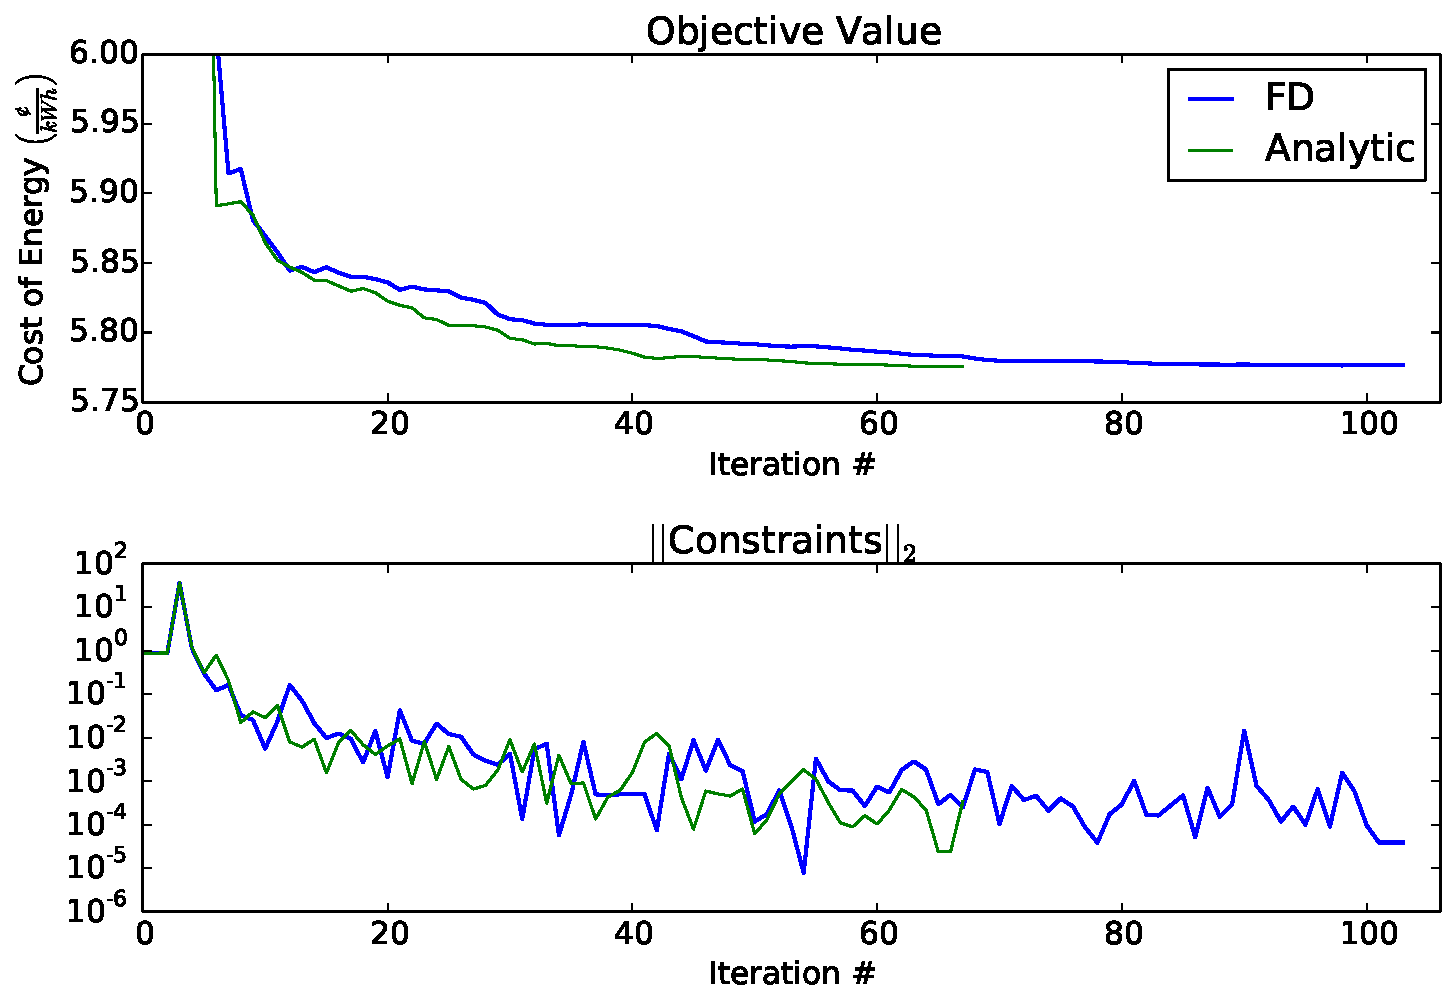
\includegraphics[width=0.95\textwidth]{images/wt_opt_progress}
          \caption{Comparison between optimization performance and finite-difference and analytic gradients.}
          \label{fig:wt-opt-progress}
        \end{figure}




  \section{Conclusion}

      Different types of sparsity exist throughout a multidisciplinary design problem. Certain
      disciplines may not be relevant to all objectives and constraints, not all variables within a discipline will
      be relevant, and the Jacobians for any given discipline may be sparse. We implemented a graph-based
      approach to identify the sparsity in any given formulation using a graph structure designed to allow for
      efficient usage even with millions of variables. We further developed a flexible API
      that allowed disciplines to declare their partial derivatives to OpenMDAO in a manner that
      takes full advantage of any sparsity within its Jacobian. Through the combination of the graph based
      method to find the minimum set of relevant variables and the flexible API OpenMDAO was able to take full
      advantage of the sparsity at all levels in a problem formulation.

      The approach was applied to two different design problems, each with unique characteristics that
      tested different aspects of the method. The small satellite design problem had millions of variables and used all analytic adjoint derivatives.
      This problem would have been very difficult to solve without analytic derivatives because of its large design spaces, however assembling the
      system-level derivatives would have been challenging to do by hand thanks to the large number of analyses involved.
      The results from the optimization of the small satellite reveal that the implementation scales well with increasing
      number of variables and a significant computational cost benefit was obtained by taking advantage of
      sparsity in the problem formulation. The wind turbine design problem had a smaller design space, a
      significantly more complex problem formulation, and used a combination of finite-difference and analytic
      gradients. The problem was solved with forward gradients because it had more constraints than design variables.
      The optimization results demonstrated OpenMDAO's ability to solve highly nested problems with coupled derivatives.
      In addition, they showed a gain in computational efficiency by applying analytic derivatives, even though some major
      analyses still required finite differencing.

      The combined results from the two design problems clearly demonstrate the value of the approach presented here: efficient and
      automatic computation of system-level derivatives, given partial derivatives from the discipline analyses
      even for very large problems. It also allows analyses with and without analytic derivatives to be used effectively
      within the same model.


  \section{Acknowledgments}

      This work was supported by the NASA Fundamental Aeronautics Program, Aeronautical Sciences Project.
      The authors would like to thank Dae Young Lee and Prof. James W. Cutler from the University of Michigan
      for contributing to the development of the analyses used in the small satellite design problem.  The authors also gratefully acknowledge the contributions of Katherine Dykes, Yi Guo, and Ryan King from the National Renewable Energy Laboratory for their development efforts on the wind turbine nacelle and cost models.

  \bibliography{references}


\end{document}
